% LTEX: enabled=false
% **************************************************
% Document Class Definition
% **************************************************
\documentclass[%
    paper=A4,               % paper size --> A4 is default in Germany
    twoside=true,           % onesite or twoside printing
    openany,              % doublepage cleaning ends up right side
    parskip=full,           % spacing value / method for paragraphs
    chapterprefix=true,     % prefix for chapter marks
    11pt,                   % font size
    headings=normal,        % size of headings
    bibliography=totoc,     % include bib in toc
    listof=totoc,           % include listof entries in toc
    titlepage=on,           % own page for each title page
    captions=tableabove,    % display table captions above the float env
    chapterprefix=false,    % do not display a prefix for chapters
    appendixprefix=false,   % but display a prefix for appendix chapter
    draft=false,            % value for draft version
]{scrreprt}%

\usepackage[utf8]{inputenc}
\usepackage[T1]{fontenc}
\usepackage[english]{babel}

\usepackage{graphicx}
% format numbers
\usepackage{siunitx}
%https://tex.cloud.uni-hannover.de/project/6677e7bc8f12321099572893
\sisetup{
    locale=DE,
    group-digits = integer,
    round-mode = places,
    round-precision = 3,
    round-pad = false
}
% better itemize and enumerate
\usepackage{enumitem}
% \setlist[itemize]{nosep, label=-} 
% \setlist[enumerate,1]{label=\alph*)}
% enables \enquote command for better quotation
\usepackage{csquotes}
\usepackage[nolist,nohyperlinks]{acronym}

% \usepackage{tabularx} 
% \usepackage{ragged2e}
% \newcolumntype{L}{>{\RaggedRight}X}
% \newcolumntype{R}{>{\RaggedLeft}X}
% \newcolumntype{C}{>{\centering\arraybackslash}X}
% \newcommand{\hrc}[1]{\multicolumn{1}{C}{#1}}
% \usepackage{multirow}
% \usepackage{booktabs}

% All floats are flushed before the next section
\usepackage[section]{placeins}
% code typesetting
\usepackage{listings}

\usepackage{biblatex}
\addbibresource{literature.bib}

\usepackage[hidelinks]{hyperref}
\hypersetup{
    pdftitle={Developing Interpretable Style Vectors to Steer Large Language Models towards Group-Specific Explanation Generation},
    pdfsubject={Master Thesis},
    colorlinks=false,
    pdfpagemode=UseNone,
    pdfauthor={Janek Prange}
}


% **************************************************
% Information and Commands for Reuse
% **************************************************
\newcommand{\thesisTitle}{Developing Interpretable Style Vectors to Steer Large Language Models towards Group-Specific Explanation Generation}
\newcommand{\thesisName}{Janek Prange}
\newcommand{\matrikelnummer}{10031585}
\newcommand{\thesisSubject}{Master's Thesis}
\newcommand{\thesisDate}{June 5, 2025}
% \newcommand{\thesisVersion}{My First Draft}

\newcommand{\thesisFirstReviewer}{Prof. Dr. rer. nat. Henning Wachsmuth}
\newcommand{\thesisFirstReviewerUniversity}{\protect{Leibniz University Hannover}}
\newcommand{\thesisFirstReviewerDepartment}{Electrical Engineering and Computer Science}

\newcommand{\thesisSecondReviewer}{Prof. Dr. Ralph Ewerth}
\newcommand{\thesisSecondReviewerUniversity}{\protect{Leibniz University Hannover}}
\newcommand{\thesisSecondReviewerDepartment}{Electrical Engineering and Computer Science}

\newcommand{\thesisFirstSupervisor}{M.Sc. Leandra Fichtel}
% \newcommand{\thesisSecondSupervisor}{}

\newcommand{\thesisUniversity}{\protect{Leibniz University Hannover}}
\newcommand{\thesisUniversityDepartment}{Electrical Engineering and Computer Science}
\newcommand{\thesisUniversityInstitute}{Institute of Artificial Intelligence (LUH-AI)}
\newcommand{\thesisUniversityGroup}{Natural Language Processing (NLP)}
\newcommand{\thesisUniversityCity}{Hannover}
\newcommand{\thesisUniversityStreetAddress}{Welfengarten 1}
\newcommand{\thesisUniversityPostalCode}{30167}


% **************************************************
% Debug LaTeX Information
% **************************************************
%\listfiles


% Everything supposed to be used in equation mode?
% use in preamble: \input{macros_DAC.tex}

% Necessary packages for definitions
\usepackage{amsmath}
\usepackage{mathtools}  % for :=
\usepackage{amsfonts} 

\newcommand{\code}[1]{\small{\texttt{#1}}} 

%beginmacros

%--------- General Math Notation
\DeclareMathOperator*{\E}{\mathbb{E}}           % Expectation as a math operator
\DeclareMathOperator*{\expectation}{\mathbb{E}} % Expectation as a math operator
\renewcommand{\vec}[1]{\mathbf{#1}}             % Bold emphasis for vectors
\DeclareMathOperator*{\argmin}{arg\,min}        % Argmin
\DeclareMathOperator*{\argmax}{arg\,max}        % Argmax
\newcommand{\natnums}{{\mathbb{N}}}              % Notation for set of natural numbers
\newcommand{\realnums}{{\mathbb R}}             % Notation for set of real numbers
\newcommand{\extset}[2]{\{#1 \; | \; #2\}}      % Set of a given b. Renders {{a | b}}.    
\newcommand{\ddfrac}[2]{\frac{\displaystyle #1}{\displaystyle #2}}    % Double Display Fraction, forces large displays for everything in numerator and denominator

\newcommand{\diff}{\mathop{}\!\mathrm{d}}       % ???????
\newcommand{\transpose}[0]{{\textrm{\tiny{\sf{T}}}}} % Transpose T. Usage: $A^\transpose$
\newcommand{\norm}{{\mathcal{N}}}               % Normal distribution
\newcommand{\normaldist}{{\mathcal{N}}}         % Normal distribution
\newcommand{\iter}[2][\bocount]{{#2}^{(#1)}}    % Iteration specific instance of variable/function/anything

%-- Stochastic
\newcommand{\pdf}{\phi}                         % Standard Normal PDF
\newcommand{\cdf}{\Phi}                         % Standard Normal CDF
\newcommand{\mean}{\mu}                         % Mean
\newcommand{\stddev}{\sigma}                    % Standard Deviation
\newcommand{\variance}{\sigma^2}                % Variance
\newcommand{\noise}{\nu}                        % Noise
\newcommand{\given}[1][]{\:#1\vert\:}           % Conditional Probability "Given That" Relation, source: https://tex.stackexchange.com/a/141685/205886
\newcommand{\prob}[0]{p}                        % Probability p
\newcommand{\Prob}[0]{P}                        % Probability distribution P


%------- Notation for Configuration(s)

\newcommand{\confspace}[0]{\pmb{\Lambda}}       % Configuration space of parameters
\newcommand{\conf}[0]{\pmb{\lambda}}            % Configuration of parameters
%\newcommand{\bx}[0]{\conf}                     % Configuration of parameters
\newcommand{\hyperparam}{\lambda}               % Single hyperparameter of configuration
\newcommand{\hyperparami}[1][i]{{\hyperparam}_{#1}}   % Single hyperparameter within a hyperparameter configuration
\newcommand{\confinc}[0]{\pmb{\hat{\lambda}}}   % Incumbent configuration
%\newcommand{\confI}[1]{{\conf}^{(#1)}}      % Configuration corresponding to a given iteration -- better use \iter!
\newcommand{\confdef}[0]{{\conf}_{\text{def}}}  % Default configuration
\newcommand{\incumbent}[1][\bocount]{\iter[#1]{\confinc}}   % Incumbent configuration
\newcommand{\confincfin}{\incumbent[\bobudget]} % Final incumbent configuration (at end of run)
\newcommand{\confopt}[0]{{\conf}^*}             % Optimal configuration


%------- Notation for Cost, Risk, Loss, Performance Metric or Objective Functions

\newcommand{\loss}[0]{\mathcal{L}}              % Loss
\newcommand{\risk}{\mathcal{R}}                 % Risk
\newcommand{\riskemp}{\mathcal{R}_{\text{emp}}} % Empirical risk
\newcommand{\cost}[0]{c}                        % Cost
\newcommand{\costi}[1]{c^{(#1)}}                % Cost of instance/identifier
\newcommand{\objF}{F}                           % Family of objective functions
\newcommand{\func}[0]{f}                        % Function
\newcommand{\perfdomain}[0]{\mathbb{R}}         % Performance domain


%------- Notation for Algorithms
\newcommand{\algo}[0]{A}                        % One algorithm
\newcommand{\algos}[0]{\mathbf{A}}              % Set of algorithms    


\newcommand{\feat}[0]{\x_{\text{meta}}}                 % Meta features
\newcommand{\feats}[0]{\mathcal{X}_{\text{meta}}}       % Set of meta features


%------- Notation for Machine Learning
\newcommand{\dset}[0]{\mathcal{D}}                          % Dataset (instance)
\newcommand{\dsetmeta}[0]{\dset_{\text{meta}}}              % Dataset: meta
\newcommand{\dsettrain}[0]{\dset_{\text{train}}}            % Dataset: train
\newcommand{\dsetval}[0]{\dset_{\text{val}}}                % Dataset: val
\newcommand{\dsettest}[0]{\dset_{\text{test}}}              % Dataset: test
\newcommand{\x}[0]{\mathbf{x}}                              % Input vector x
\newcommand{\y}[0]{y}                                       % Output y
\newcommand{\xI}[1]{\mathbf{x}^{(#1)}}                      % i-th component of input
\newcommand{\yI}[1]{y^{(#1)}}                               % i-th component of output
\newcommand{\fx}{f(\mathbf{x})}                             % f(x), continuous prediction function
\newcommand{\Hspace}{\mathcal{H}}                           % hypothesis space where f is from
\newcommand{\fh}{\hat{f}}                                   % f hat, estimated prediction function


%------- Notation for Deep Learning
\newcommand{\weights}[0]{\mathbf{\theta}}                   % Weights of neural network
\newcommand{\metaweights}[0]{\phi}                          % Weights of a meta-network


%------- Notation for AutoML
\newcommand{\portfolio}[0]{\mathbf{P}}                      % Portfolio
\newcommand{\schedule}[0]{\mathcal{S}}                      % Schedule
\newcommand{\hist}[0]{\dset_{\text{hist}}}                  % History


%------- Notation for Bayesian Optimization
%-- Components
\newcommand{\GP}{\mathcal{G}}                   % Gaussian Process
\newcommand{\kernel}{\kappa}                    % Kernel
\newcommand{\acq}{u}                            % Acquisition Function
\newcommand{\constraintg}{g}                    % Constraint function
\newcommand{\surro}[0]{\hat{\cost}}             % Surrogate model

%-- Loop
\newcommand{\bocount}{t}                        % BO loop counter
\newcommand{\bobudget}{T}                       % BO loop counter max, the counter runs from 1 to this value
\newcommand{\obs}[1][\conf]{\cost({#1})}        % BO loop observation
\newcommand{\obsspace}{\mathcal{Y}}             % BO loop observation space
\newcommand{\bonextobs}{\obs[\iter{\conf}]}     % BO loop next observation
\newcommand{\bonextsample}{\iter{\conf}}        % BO loop next selected sample

%-- Dataset
\newcommand{\dsetHPOdef}{{\langle \bonextsample,\,\bonextobs \rangle}_{\bocount=1}^{\bobudget}}     % Observed cost for selected configurations during BO run


%------- Notation for Reinforcement Learning
%-- Markov Decision Process with Components
\newcommand{\MDP}[0]{M}                       % MDP (Markov Decision Process)
\newcommand{\statespace}[0]{\mathcal{S}}                % State space
\newcommand{\state}[0]{s}                               % State
\newcommand{\statet}[1][t]{\state_{#1}}                 % State at time t
\newcommand{\actionspace}[0]{\mathcal{A}}               % Action space
\newcommand{\actionrl}[0]{a}                            % Action
\newcommand{\transdomain}[0]{\mathcal{T}}               % Transition domain (probability distribution of algorithm state transitions)
\newcommand{\trans}[0]{t}                               % Transition
\newcommand{\rewards}[0]{\mathcal{R}}                   % Reward function
\newcommand{\reward}[0]{r}                              % Reward

\newcommand{\policies}[0]{\mathbf{\Pi}}                 % Policies
\newcommand{\policy}[0]{\pi}                            % Policy
\newcommand{\policyopt}[0]{{\policy}^*}                 % Optimal policy

\newcommand{\discount}[0]{\gamma}                       % Discount rate
\newcommand{\valueS}[0]{\mathcal{V}}                    % State value function
\newcommand{\valueSip}[1][\inst]{\valueS^{\policy}_{#1}} % State value function under policy pi and instance i
\newcommand{\Qfunc}[0]{\mathcal{Q}}                     % State action value function (Q)
\newcommand{\Qfuncip}[1][\inst]{\Qfunc^{\policy}_{#1}}  % State action value function (Q) under policy pi and instance i

\newcommand{\egreedy}[0]{$\epsilon$-greedy}             % $\egreedy$ 

\newcommand{\trajectory}{\tau}                          % Trajectory
\newcommand{\episode}[0]{\mathcal{E}}                  % Episode
\newcommand{\expreturn}[0]{G}                           % Expected return
\newcommand{\cutoff}[0]{\kappa}                         % Cutoff kappa


%-- Dynamic Algorithm Configuration (DAC)
\newcommand{\inst}[0]{i}                    % One instance
\newcommand{\insts}[0]{\mathcal{I}}         % Set of instances
\newcommand{\insti}[1]{i^{(#1)}}            % Numbered instance. Usage: $\insti{3}$ for 3rd instance.

\newcommand{\cMDP}[0]{\mathcal{M}}                      % cMDP (contextual MDP)
\newcommand{\cMDPdef}[0]{\cMDP \coloneqq \{\MDPi\}_{\inst \sim \insts}} % cMDP: Definition as set of MDPs per instance
\newcommand{\MDPi}[0]{\MDP_\inst}                       % MDP of one instance
\newcommand{\MDPidef}[0]{\MDPi \coloneqq (\statespace, \actionspace, \transdomaini, \rewardsi)}  % MDP: Definition as tuple for one instance

\newcommand{\transdomaini}[0]{\transdomain_\inst}       % Transitions (instance-specific)
\newcommand{\rewardsi}[0]{\rewards_\inst}               % Rewards (instance-specific)    
\newcommand{\curric}[0]{\mathbf{d}}                     % Curriculum
\newcommand{\contexti}[1][i]{c_{#1}}                    % Context of instance i

\newcommand{\configspaceDAC}[0]{\Theta}                 % Configuration space
\newcommand{\configDAC}[0]{\theta}                      % Configuration
\newcommand{\hyperparamset}{H}                          % Hyperparameter set
\newcommand{\hyperparamname}[0]{h}                      % Name of hyper-/configuration parameter

%endmacros


% Regret
% Return

% **************************************************
% Document CONTENT
% **************************************************
\begin{document}

% **************************************************
% Description
% **************************************************
%\input{content/tasks_desccription/descriptionpage}


% --------------------------
% rename document parts
% --------------------------
%\renewcaptionname{ngerman}{\figurename}{Abb.}
%\renewcaptionname{ngerman}{\tablename}{Tab.}
\renewcaptionname{english}{\figurename}{Figure}
\renewcaptionname{english}{\tablename}{Table}

% --------------------------
% Front matter
% --------------------------
\pagenumbering{roman}			% roman page numbing (invisible for empty page style)
\pagestyle{empty}				% no header or footers
% !TeX root = ..\..\thesis.tex
%
% ------------------------------------  --> cover title page
\begin{titlepage}
  % \pdfbookmark[0]{Cover}{Cover}
  \flushright
  \hfill
  \vfill
  {\LARGE\thesisTitle \par}
  \rule[5pt]{\textwidth}{.4pt} \par
  {\Large\thesisName}
  \vfill
  \textit{\large\thesisDate} \\
  % Version: \thesisVersion
\end{titlepage}



% ------------------------------------  --> main title page

\begin{titlepage}

  % \pdfbookmark[0]{Titlepage}{Titlepage}
  \tgherosfont

  \begin{figure}
    \begin{minipage}[t]{8.5cm}
      
\includegraphics[height=1.5cm]{figures/LUHAI_banner.png}\\
      \textsf{\small{Electrical Engineering and Computer Science,\\
          Institute of Artificial Intelligence (LUHAI)\\
          %		\hspace*{1.3cm}Institute of Computer Science\\
          Appelstraße 9a \\
          30167 Hannover
        }}
    \end{minipage}
    \hfill
    \begin{minipage}[t]{4.7cm}
      
\includegraphics[scale=0.3]{figures/luh_logo_grey.pdf}\\
      \textsf{%Institute of Computer Science\\
        \hspace*{0.1cm}\small{}
      }
    \end{minipage}
  \end{figure}

  \centering
  %\textsf{\thesisUniversityDepartment} \\
  %\textsf{\thesisUniversityInstitute} \\
  %\textsf{\thesisUniversityGroup} \\

  \vfill
  {\large \thesisSubject} \\[5mm]
  {\LARGE \color{ctcolortitle}\textbf{\thesisTitle} \\[10mm]}
  {\Large \thesisName} \\

  \vfill
  \begin{minipage}[t]{.27\textwidth}
    \raggedleft
    \textit{1. Reviewer}
  \end{minipage}
  \hspace*{15pt}
  \begin{minipage}[t]{.65\textwidth}
    {\Large \thesisFirstReviewer} \\
    {\small \thesisFirstReviewerDepartment} \\[-1mm]
    {\small \thesisFirstReviewerUniversity}
  \end{minipage} \\[5mm]
  \begin{minipage}[t]{.27\textwidth}
    \raggedleft
    \textit{2. Reviewer}
  \end{minipage}
  \hspace*{15pt}
  \begin{minipage}[t]{.65\textwidth}
    {\Large \thesisSecondReviewer} \\
    {\small \thesisSecondReviewerDepartment} \\[-1mm]
    {\small \thesisSecondReviewerUniversity}
  \end{minipage} \\[10mm]
  \begin{minipage}[t]{.27\textwidth}
    \raggedleft
    \textit{Supervisor}
  \end{minipage}
  \hspace*{15pt}
  \begin{minipage}[t]{.65\textwidth}
    \thesisFirstSupervisor\ %and \thesisSecondSupervisor
  \end{minipage} \\[10mm]

  % Date of Submission: \thesisDate \\
  \vspace{2cm}
  \begin{flushright}
    Date of Submission: \thesisDate \\
  \end{flushright}

  % 
\includegraphics[width=210mm,height=70mm]{figures/castle.png}
  % Set the position of the banner at the bottom of the page
  \begin{textblock*}{210mm}(0mm,297mm-70mm) % Set X and Y coordinates. 297mm is the height of A4 paper
    % Include your banner image
    
\includegraphics[width=210mm,height=70mm]{figures/castle.png}
  \end{textblock*}
\end{titlepage}


% ------------------------------------  --> lower title back for single page layout
\hfill
\vfill
{
  \small
  \textbf{\thesisName} \\
  \textit{\thesisTitle} \\
  \thesisSubject, \thesisDate \\
  \begin{tabular}[t]{@{} r @{ } l @{}}
    Reviewers: & \thesisFirstReviewer  \\
    and        & \thesisSecondReviewer \\
  \end{tabular} \\
  \begin{tabular}[t]{@{} r @{ } l @{}}
    Supervisor: & \thesisFirstSupervisor \\
    % Supervisors: & \thesisFirstSupervisor  \\
    % and          & \thesisSecondSupervisor \\
  \end{tabular} \\[1.5em]
  \textbf{\thesisUniversity} \\
  \textit{\thesisUniversityGroup} \\
  \thesisUniversityInstitute \\
  \thesisUniversityDepartment \\
  \thesisUniversityStreetAddress \\
  \thesisUniversityPostalCode\ \thesisUniversityCity
}
		% INCLUDE: all titlepages
\cleardoublepage

% !TeX root = ..\..\thesis.tex
%
%************************************************
% Declaration
%************************************************
\pdfbookmark[0]{Declaration}{Declaration}
\chapter*{Declaration}
\label{sec:declaration}
\thispagestyle{empty}

\justifying{Hiermit erkläre ich, dass ich die vorliegende Arbeit selbstständig verfasst, keine anderen als die
  angegebenen Quellen und Hilfsmittel verwendet sowie die aus fremden Quellen direkt oder
  indirekt übernommenen Stellen/Gedanken als solche kenntlich gemacht habe.}

\vspace{2cm}

\begin{table}[h]
  \begin{tabular}{@{}p{5cm}p{5cm}@{}}
    \thesisUniversityCity, \thesisDate, & \rule{5cm}{0.4pt} \\[0.01cm]
                                        & \thesisName
  \end{tabular}
\end{table}




%*****************************************
%*****************************************

\clearpage

\pagestyle{plain}				% display just page numbers
\section{Abstract}		% INCLUDE: the abstracts (english and german)
\cleardoublepage
%
% % !TeX root = ..\..\thesis.tex
%

%\documentclass[../main.tex]{subfiles}

%\begin{document}
\pdfbookmark[0]{Acknowledgement}{Acknowledgement}
\chapter*{Acknowledgement}
\label{sec:acknowledgement}
\vspace*{-10mm}



%\end{document} % INCLUDE: acknowledgement
% \cleardoublepage
%
% !TeX root = ..\..\thesis.tex

\begin{acronym}[ActAdd] % the option is the longest short form to properly format the list of acronyms
  \acro{llm}[LLM]{large language model}
  \acro{lisa}[LISA]{Linguistically Interpretable Style Attribute}
  \acro{sfam}[SFAM]{Style Feature Agreement Model}
  \acro{actadd}[ActAdd]{Activation Addition}
  \acro{stel}[STEL]{STyle EvaLuation framework}
\end{acronym} % INCLUDE: acronyms
\cleardoublepage
%
\currentpdfbookmark{\contentsname}{toc}
\setcounter{tocdepth}{2}		% define depth of toc
\tableofcontents				% display table of contents
\cleardoublepage

% --------------------------
% Body matter
% --------------------------
\newcounter{content}
\setcounter{content}{
    \value{page}}               % save value of first content page (is reset by \pagenumbering)
\pagenumbering{arabic}			% arabic page numbering
\setcounter{page}{
    \value{content}}            % set page counter to value saved above
\pagestyle{scrheadings}     	% fancy header and footer

\newcommand{\styleVectorSize}{768}
\newcommand{\styleEmbeddingSize}{768}
% minimum cosine similarity for sentences to be in the same cluster
\newcommand{\minCosineSimilarity}{0.85}
% the maximum similarity that two clusters can have to be selected as a style attribute
\newcommand{\maxCosineSimilarity}{0.7}
% the maximum ratio of groups a cluster is used to describe for it to be selected
\newcommand{\clusterMaxGroupRatio}{\SI{60}{\percent}}
% the maximum number of clusters after the first selection step
\newcommand{\maxClustersFirstSelection}{10000}
% the minimum number of knowledge prompts
\newcommand{\minNumKnowledgePrompts}{50}
% the number of target prompts
\newcommand{\numPrompts}{92}
\newcommand{\numTargetPrompts}{84}
\newcommand{\numOpenPrompts}{6}
\newcommand{\numKnowledgePrompts}{2}

\newcommand{\numGroups}{11}


% number of answers used for the style vector creation
\newcommand{\numAnswersStyleVector}{5500}
% number of style descriptions
\newcommand{\numStyleDescriptions}{0}
% number of style sentences
\newcommand{\numStyleSentences}{0}
% number of style sentences from style prompts
\newcommand{\numStyleSentencesStyle}{0}
% number of style sentences from knowledge prompts
\newcommand{\numStyleSentencesKnowledge}{0}
% number of clusters
\newcommand{\numClusters}{0}
% number of clusters from style prompts
\newcommand{\numClustersStyle}{0}
% number of clusters from knowledge prompts
\newcommand{\numClustersKnowledge}{0}


\chapter{Introduction}
\label{sec:introduction}
Textual information plays a crucial role in daily life, appearing in various contexts, such as educational environments, news articles, entertainment media, and social media platforms. As noted in \citet{wegmannSameAuthorJust2022}, an important aspect of text is not only the message it conveys, but also the style in which it is presented. The style of a text significantly influences its reception, shaping how effectively the message is understood and how well it is accepted by the audience.

Stylistic features also serve analytical purposes; for instance, they can be used to identify the author of a text, as shown in \citet{alshomaryLatentSpaceInterpretation2024}, or to attribute the text to a particular group of individuals, as demonstrated by \citet{10.1007/978-3-642-29047-3_27}. Previous work, such as that of \citet{zhu-etal-2024-styleflow, ijcai2020p526, wegmannSameAuthorJust2022}, has highlighted the importance of style in textual analysis.

However, automating stylistic investigations with machine learning poses several challenges. One significant issue is the complexity and time-consuming nature of manual style annotations. Additionally, it is difficult to generate parallel datasets that include positive and negative examples for each stylistic label.

Because supervised learning methods rely on annotated data for training, state-of-the-art style representation methods tend to use unsupervised learning techniques. % TODO: citation
While effective, these methods often produce style embeddings that are difficult to interpret, which makes it harder to verify their quality and apply them to other tasks effectively.

To address these limitations, this thesis introduces interpretable attribute vectors based on the methodology proposed by \citet{patelLearningInterpretableStyle2023}. Figure~\ref{fig:attributeVector} illustrates the composition of these vectors. Each dimension of the vector corresponds to a real-world concept, and the associated value, ranging from \num{0} to \num{1}, indicates the extent to which a text aligns with the specified attribute.

\begin{figure}[ht]
  \begin{center}
    \begin{tikzpicture}[
  every node/.style={font=\sffamily},
  box/.style={draw, thick, minimum width=2.8cm, minimum height=1cm,
      rounded corners=5pt, top color=white, bottom color=purple!10!orange!20},
  arrow/.style={-{Latex[length=3mm]}, thick},
  label/.style={align=center, font=\small},
  annotation/.style={draw=none, align=center, font=\small}
  ]

  % Top text
  \node (text)[align=center, text width=10cm, font=\itshape]
  {\enquote{Really really cool action movie imo. Casting is great too. It's like they were all born for their role in that movie.}};

  % LISA box
  \node (lisa) [below=of text, box, font=\bfseries] {LISA};

  % Vector representation
  \node (vectorText) [below=of lisa, align=center]
  {\num{\styleVectorSize}-dimensional interpretable attribute vector};
  \node (vector) [below=0cm of vectorText, align=center] {\Large $\left[ 0.889,\ \dots,\ \pmb{0.613},\ \dots,\ \pmb{1.000},\ \dots,\ 0.949 \right]$};


  % Annotations
  \node (rep) [annotation, below left=1cm and -2cm of vector]
  {The author is\\repeating words.};

  \node (comp) [annotation, below right=1cm and -2cm of vector]
  {The author is\\complimentary.};

  % Arrow to LISA
  \draw[arrow] (text) -- (lisa);
  % Arrow to vector
  \draw[arrow] (lisa) -- (vectorText);
  % Arrows from vector components
  \draw[-{Latex[length=2mm]}, thick] ([xshift=-1.3cm]vector.south) -- (rep.north);
  \draw[-{Latex[length=2mm]}, thick] ([xshift=1.3cm]vector.south) -- (comp.north);
\end{tikzpicture}

    \caption{An example of a \num{\styleVectorSize}-dimensional attribute vector that was generated with the method presented in this thesis.} % TODO: more caption?
    \label{fig:attributeVector}
  \end{center}
\end{figure}

While state-of-the-art methods primarily focus on stylistic features for tasks such as authorship attribution, as shown in works by \citet{alshomaryLatentSpaceInterpretation2024, patelLearningInterpretableStyle2023, konenStyleVectorsSteering2024, zhu-etal-2024-styleflow}, other types of author-related attributes can complement these stylistic analyses. One such attribute is the author's background knowledge or experience, referred to as knowledge attributes. % TODO: why is knowledge important? citation
The interpretable attribute vector developed in this thesis therefore includes both stylistic and knowledge-related dimensions.

In addition to their relevance in tasks such as authorship attribution, group membership detection, or text classification more generally, these representations are also applicable in text generation, which is one of the most prominent applications in contemporary natural language processing. \Acp{llm}, which are based on the transformer architecture as introduced in \citet{NIPS2017_3f5ee243}, are widely used tools for generating natural language text. In recent years, \acp{llm} have been used for a wide range of tasks, including providing explanations for various topics and concepts.

As more users depend on \acp{llm}, new challenges emerge beyond ensuring the factual correctness of the generated explanations. One such challenge involves tailoring the language and conceptual content of the explanation to suit the linguistic style and background knowledge of the target audience. For instance, an explanation suitable for a Ph.D. student might be inappropriate for a middle school student, and vice versa. Style and knowledge representations can be instrumental in aligning the linguistic output with the expectations and comprehension levels of different user groups to produce the best explanations for all audiences.


\section{Problem Statement}
\label{sec:introduction:problemStatement}

Previous research has demonstrated that existing methods are highly effective for authorship attribution tasks. These approaches identify and distinguish individual writing styles, enabling the attribution of anonymous texts to specific authors with a high degree of accuracy. However, the goal of this thesis is to adapt and extend these techniques to address a related yet distinct challenge: group membership detection.

Though similar in concept, group membership detection differs from authorship attribution in significant ways. Like authorship attribution, group membership detection relies on distinguishing characteristics in the way texts are written. Groups often exhibit unique stylistic features that can serve as indicators of group identity. However, the underlying data structure presents a key distinction. Authorship attribution typically involves many authors, each of whom contributes a small number of texts. In contrast, group membership detection usually involves only a few groups, each of which provides a relatively large volume of textual data. This fundamental difference in data composition requires new approaches tailored specifically to group detection.

\begin{description}
  \item[Research Question 1] How well are the interpretable style representations suited to detect the group membership of different authors?
\end{description}

To investigate this question, this thesis extends the interpretable style representation model proposed by \citet{patelLearningInterpretableStyle2023}. The extension involves augmenting the existing style vector with additional knowledge-based attributes. These attributes capture essential information such as the experience level and background knowledge of the authors, which are factors that can vary significantly between groups. As these knowledge characteristics influence how individuals express ideas in writing, their inclusion has the potential to enhance the model's ability to differentiate between groups.

\begin{description}
  \item[Research Question 1.1] Does the interpretable style representation benefit from knowledge attributes in addition to style attributes?
\end{description}

While the task of detecting group membership is valuable in itself, as \aclp{llm} are becoming more popular, the ability to use them to generate group-specific explanations has gained increasing relevance. \acp{llm} are used in many applications to explain concepts to a large variety of groups of people. While the factual correctness of these explanations is important, the comprehensibility of the explanation is increased if the model can reflect the style and background knowledge of the recipient of the explanation. This thesis compares different steering methods and how the interpretable attribute vector that is presented in the first part of the thesis can contribute to existing methods for steering \ac{llm} outputs to better align with group-specific characteristics.

\begin{description}
  \item[Research Question 2] What is the best way to generate group-specific explanations from style representations?
\end{description}

To address this question, several steering methods for \acp{llm} will be examined. The initial focus will be on system prompt engineering, a widely used and accessible method for influencing model behavior. In particular, the thesis explores how the interpretable attribute vector can be used to guide the construction of system prompts that produce group-specific outputs. This includes formulating prompts to include dimensions of the interpretable attribute vector that are particularly relevant to a specific group.

\begin{description}
  \item[Research Question 2.1] Can the attribute vector presented in this thesis be used to improve existing steering methods that change the system prompt?
\end{description}

Despite its popularity, steering through system prompt modification has the limitation that it does not allow for fine-grained control over the steering. While it can guide the model in a general direction, it lacks the capacity to precisely modulate the strength of the steering effect.

To overcome this limitation, this thesis introduces a novel method for fine-grained steering that manipulates the activation space of the \ac{llm}. This technique involves altering the model's internal representations after specific layers, steering the activations toward particular conceptual directions that correspond to the dimensions of the interpretable attribute vector. This method builds upon recent research in activation-based model manipulation, including the work of \citet{konenStyleVectorsSteering2024,turnerActivationAdditionSteering2024,rimsky-etal-2024-steering}.

\begin{description}
  \item[Research Question 2.2] Can the newly proposed method of steering an \acs{llm} by manipulating its activation space be used to improve existing steering methods?
\end{description}


\section{Goals of the thesis}
\label{sec:introduction:goals}
\newlength{\maxstretch}
\setlength{\maxstretch}{0pt plus 1fill}
This thesis is guided by the research questions defined in Section~\ref{sec:introduction:problemStatement} and describes a continuous process. This process begins with preparing input data and ends with generating group-specific outputs from a steered model. Each goal contributes to the development of a framework for identifying group membership and steering language model behavior accordingly.

\begin{description}
  \item[Automatic Creation of an Annotated Synthetic Dataset]
        Annotating a large text corpus with diverse style and knowledge attributes is a difficult and time-consuming task. This challenge is amplified by the need for diverse attributes that are not bound to predefined topics. To address this issue, the first goal of this thesis is to create a synthetic dataset through an automated process based on the work presented by \citet{patelLearningInterpretableStyle2023}. This dataset will contain group-specific explanations, each annotated with corresponding style and knowledge attributes.

  \item[Selecting the Dimensions of the Interpretable Attribute Vector]\hspace{\maxstretch}
        The synthetic dataset contains numerous style- and knowledge-related attributes. However, the interpretable attribute vector is limited to \num{\styleVectorSize} dimensions. Thus, the goal is to design an automatic selection process that identifies the most informative and relevant dimensions from the available attributes. This process builds upon the dimensionality selection strategy proposed by \citet{patelLearningInterpretableStyle2023}, providing a more targeted and efficient representation of group-specific characteristics.

  \item[Training of a Model that Produces the Interpretable Attribute Vector]
        With the selected attributes in place, the next goal is to train a model that can map any given text to an interpretable attribute vector. Each dimension of this vector corresponds to a specific style or knowledge attribute, with values ranging between \num{0} and \num{1}, indicating the extent to which the text exhibits each characteristic. The model is based on the architecture proposed by \citet{patelLearningInterpretableStyle2023}, which has been extended to incorporate both stylistic and knowledge-based components.

  \item[Creation of an Interpretable Attribute Embedding]\hphantom{at}
        Although the interpretable attribute vector is structured, its dimensions are not normalized. This limits the ability to directly compare different vectors. To address this issue, the model from the previous step is extended with an embedding head based on the approach presented by \citet{patelLearningInterpretableStyle2023}. This component generates normalized embeddings from the interpretable vectors that are suitable for group membership detection. These embeddings enable meaningful comparisons across texts and allow for clustering or classification of texts by group identity.

  \item[Steering a Large Language Model with System Prompt Engineering]\hspace{\maxstretch}
        This goal addresses research question 2.1 and explores how the interpretable attribute vector can improve system prompt engineering techniques for \acp{llm}. Different prompt construction strategies are designed and evaluated, with a focus on integrating the most relevant attribute dimensions for a target group. The goal is to generate outputs that align with the linguistic style and background knowledge of the target group by embedding these attributes into the system prompt.

  \item[Steering a Large Language Model with Activation Steering]\hphantom{i}
        The final goal of the thesis addresses research question 2.2 and proposes a novel method for activation-based steering. This method manipulates the activations at the end of each transformer layer of the \ac{llm} by injecting steering vectors that are derived from internal model activations. The steering vectors are produced by combining activation vectors corresponding to specific dimensions of the interpretable attribute vector. Furthermore, this steering method is used in conjunction with various prompt steering methods to directly compare their performance.
\end{description}

Together, these goals form a comprehensive framework for interpretable text representation and personalized language model behavior. Beginning with the creation of the synthetic dataset, the thesis develops tools for generating and leveraging interpretable style and knowledge vectors. Ultimately, these tools are applied to guide the LLMs in ways that reflect group identity and communicative needs.

\clearpage

\chapter{Background Knowledge and Related Work}
\label{sec:background}

This chapter provides an overview of the key concepts and relevant research for this thesis. The goal is to integrate the proposed approaches into the broader context of existing work and show how they contribute to the current state of research.

\section{Embeddings}
\label{sec:background:embeddings}
Embeddings form the foundation of many modern \ac{nlp} systems by providing a mathematical representation of words, texts, or other concepts in a continuous vector space, as illustrated in Figure~\ref{fig:embeddings}. These representations capture semantic relationships, enabling machines to better understand and process human language. This section provides an overview of the evolution of embedding techniques, from early static word vectors to more recent context-aware models. Additionally, it emphasizes the importance of embeddings in a variety of \ac{nlp} applications.

\begin{figure}[h!t]
  \centering
  % source: https://www.cs.cmu.edu/~dst/WordEmbeddingDemo/tutorial.html
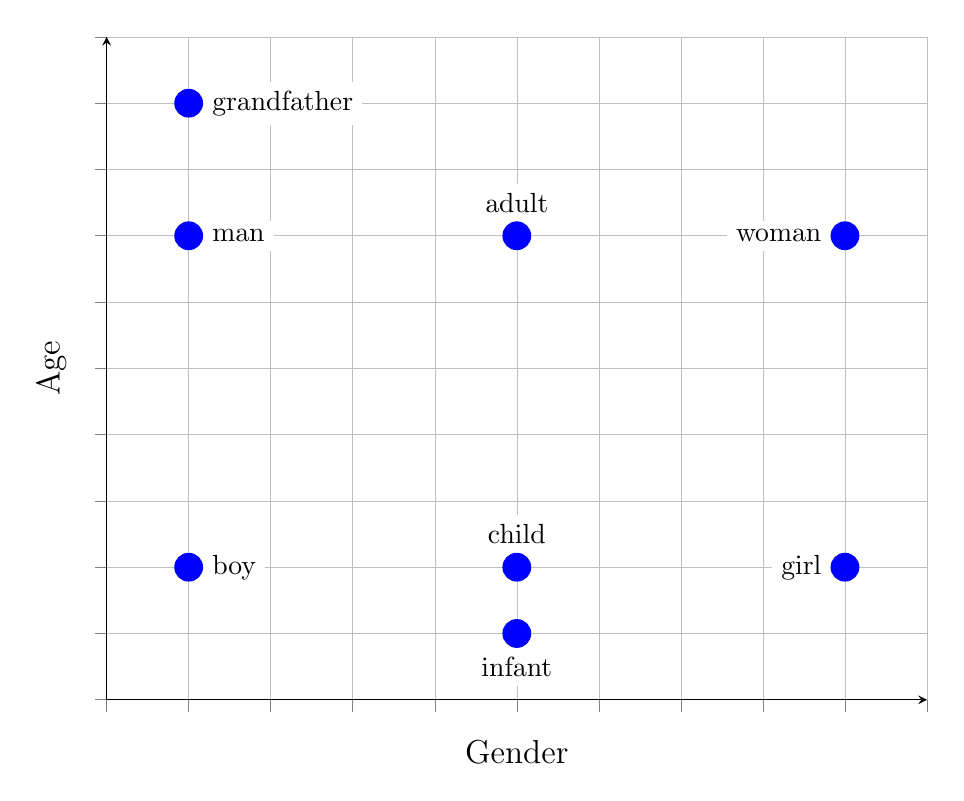
\begin{tikzpicture}
  \begin{axis}[
      width=12cm, height=10cm,
      xlabel={Gender}, ylabel={Age},
      xmin=0, xmax=10, ymin=0, ymax=10,
      xtick={0,1,...,10}, ytick={0,1,...,10},
      xticklabel={\empty}, yticklabel={\empty},
      grid=both,
      grid style={line width=.1pt, draw=gray!30},
      major grid style={line width=.2pt,draw=gray!50},
      axis lines=left,
      tick align=outside,
      enlargelimits=false,
      label style={font=\large},
      title style={font=\LARGE, yshift=1em},
      every tick label/.append style={font=\small},
    ]

    % Plot the points
    \addplot[
      only marks,
      mark=*,
      mark size=5pt,
      blue,
    ] coordinates {
        (1,9)   % grandfather
        (1,7)   % man
        (1,2)   % boy
        (5,7)   % adult
        (5,2)   % child
        (5,1)   % infant
        (9,7)   % woman
        (9,2)   % girl
      };

    % Add labels
    \node[fill=white, anchor=west, xshift=5pt, font=\normalsize] at (axis cs:1,9)  {grandfather};
    \node[fill=white, anchor=west, xshift=5pt, font=\normalsize] at (axis cs:1,7)  {man};
    \node[fill=white, anchor=west, xshift=5pt, font=\normalsize] at (axis cs:1,2)  {boy};
    \node[fill=white, anchor=south, yshift=5pt, font=\normalsize] at (axis cs:5,7)  {adult};
    \node[fill=white, anchor=south, yshift=5pt, font=\normalsize] at (axis cs:5,2)  {child};
    \node[fill=white, anchor=north, yshift=-5pt, font=\normalsize] at (axis cs:5,1)  {infant};
    \node[fill=white, anchor=east, xshift=-5pt, font=\normalsize] at (axis cs:9,7)  {woman};
    \node[fill=white, anchor=east, xshift=-5pt, font=\normalsize] at (axis cs:9,2)  {girl};
  \end{axis}
\end{tikzpicture}
  \caption[]{%
    This figure (\cite{WordEmbeddingDemo}) shows a simplified visualization of a word embedded in a semantic feature space. In such embeddings, the absolute position of words in the space is meaningless; only the relative positions of the points matter. Semantically similar words are represented by points that are located close to one another in the embedding space. Additionally, certain directions in the embedding space may correspond to real-world concepts. For instance, in this example, certain directions correspond to age or gender.

    Word embeddings are typically generated using unsupervised learning methods. Consequently, the individual dimensions of the embeddings do not explicitly correspond to interpretable, real-world concepts. This differs from the current illustration, where each axis is clearly labeled with a human-understandable attribute. Nevertheless, two key characteristics generally remain valid: embeddings that are close together tend to be semantically similar, and some directions in the embedding space can reflect meaningful concepts.}%
  \label{fig:embeddings}
\end{figure}

Early models for word representation focused on learning fixed vectors for each word, resulting in what are known as static word embeddings. These embeddings assign the same vector to a word regardless of the context in which it appears. Well-known examples of such approaches include Word2Vec (\cite{mikolovEfficientEstimationWord2013}) and GloVe (\cite{penningtonGloveGlobalVectors2014}), both of which capture semantic similarities based on word co-occurrence statistics in large text corpora.

Although static word embeddings are computationally efficient and useful in many scenarios, they are unable to account for variations in meaning across different contexts. This limitation has led to the development of contextual word embeddings, which are context-dependent. One early example is ELMo (\cite{petersDeepContextualizedWord2018}), which uses bidirectional \ac{lstm} networks to generate embeddings sensitive to surrounding words in a sentence.

More recent approaches use transformer-based architectures. Models such as BERT (\cite{devlin-etal-2019-bert}) generate deep contextual embeddings using self-attention mechanisms to model relationships between words within a given context. Contextual information is crucial because it enables models to disambiguate polysemous words. For example, the word \enquote{bank} can refer to a financial institution or the side of a river, and only contextual clues can determine the intended meaning.

These contextual embeddings have substantially improved performance across a wide variety of \ac{nlp} tasks, including question answering, named entity recognition, and machine translation. As a result, they have become essential components of modern \ac{nlp} pipelines.

\section{Stylistic Investigations}
\label{sec:background:styleInvestigations}
% TODO: write a little more about the proxy tasks; what are they, what are examples, why are they necessary
% TODO: example for learned style embedding method with citation
The objective of Stylistic Investigations is to identify an author's unique writing style independent of the content being expressed. Modern neural approaches often accomplish this by learning dense vector representations, or style embeddings, through proxy tasks. These tasks include style transfer, authorship attribution or verification, and group membership detection. Proxy tasks enable models to learn stylistic features without explicit style annotations. This is important because annotating large amounts of data is very difficult and time-consuming.

However, one drawback of learned style embeddings is that it is difficult to ensure that the representations are truly independent of the content, as noted by \citet{wegmannSameAuthorJust2022}. This complicates their application in new domains where the content may differ. Additionally, such embeddings tend to be uninterpretable, reducing their transparency and limiting their usefulness in downstream tasks.

Some approaches aim to produce interpretable embeddings to address these issues. Notable examples include the work by \citet{patelLearningInterpretableStyle2023}, who propose a method for learning attribute-based representations, and \citet{alshomaryLatentSpaceInterpretation2024}, who focus on interpreting latent embeddings. This thesis builds on and extends this line of research by proposing a new method for learning interpretable style embeddings that incorporate knowledge-related dimensions.

Other, more classical methods for stylistic analysis take a different approach. They work by manually selecting interpretable features such as the frequency of function words, syntactic structures, or punctuation counts. These features are extracted using comprehensible algorithms and can be used to construct explainable classifiers, although they may lack the nuance and representational capacity of neural embeddings.
\citet{okulskaStyloMetrixOpensourceMultilingual2023} presented Stylometrix as an example of recent work in this area. It generates interpretable style vectors based on a curated set of features. Another example is StyloAI, which was developed \citet{oparaStyloAIDistinguishingAIgenerated2024} and extracts 31 stylometric features to identify AI-generated texts using a Random Forest classifier.

The main advantages of feature-based approaches are the relevance and quality of the extracted features. However, these methods have several drawbacks. First, they require manual feature selection, which limits the range of stylistic attributes that can be captured. Additionally, these methods cannot incorporate more abstract attributes requiring a deeper understanding of the text, such as the knowledge-related features employed in this thesis.

\section{Large Language Models}
\label{sec:background:llm}

\Acfp{llm} are large-scale neural networks with billions of parameters. These models are pre-trained on massive text corpora and can perform tasks that require advanced language understanding and generation (\cite{minaeeLargeLanguageModels2025}).
\acp{llm} have brought significant advancements to the field of \acl{nlp}, achieving state-of-the-art performance in a broad range of applications. These include text generation, translation, and question answering, among many others.

The transformer architecture, introduced by \citet{NIPS2017_3f5ee243} in the seminal paper \enquote{Attention Is All You Need}, is the foundation of most modern \acp{llm}. Unlike earlier models, which relied on recurrence or convolution, the transformer architecture uses self-attention mechanisms to weigh the relevance of each word in the input sequence relative to the others. This design supports parallel processing, thereby improving training efficiency and scalability.

As shown in Figure~\ref{fig:transformerArchitecture}, the transformer follows an encoder-decoder architecture. The encoder processes the input sequence and produces a continuous representation. Then, the decoder generates the output sequence based on the encoder's output and previous outputs. There are encoder-only models, such as embedding models, that produce a representation of the input text. There are also decoder-only models that predict subsequent tokens based on previous outputs or a prompt.

This thesis will employ encoder-only models to create interpretable attribute embeddings. Decoder-only \acp{llm} will be used for the task of text generation.

\begin{figure}[ht]
  \begin{center}
    \scalebox{0.95}{
      % source: https://github.com/negrinho/sane_tikz
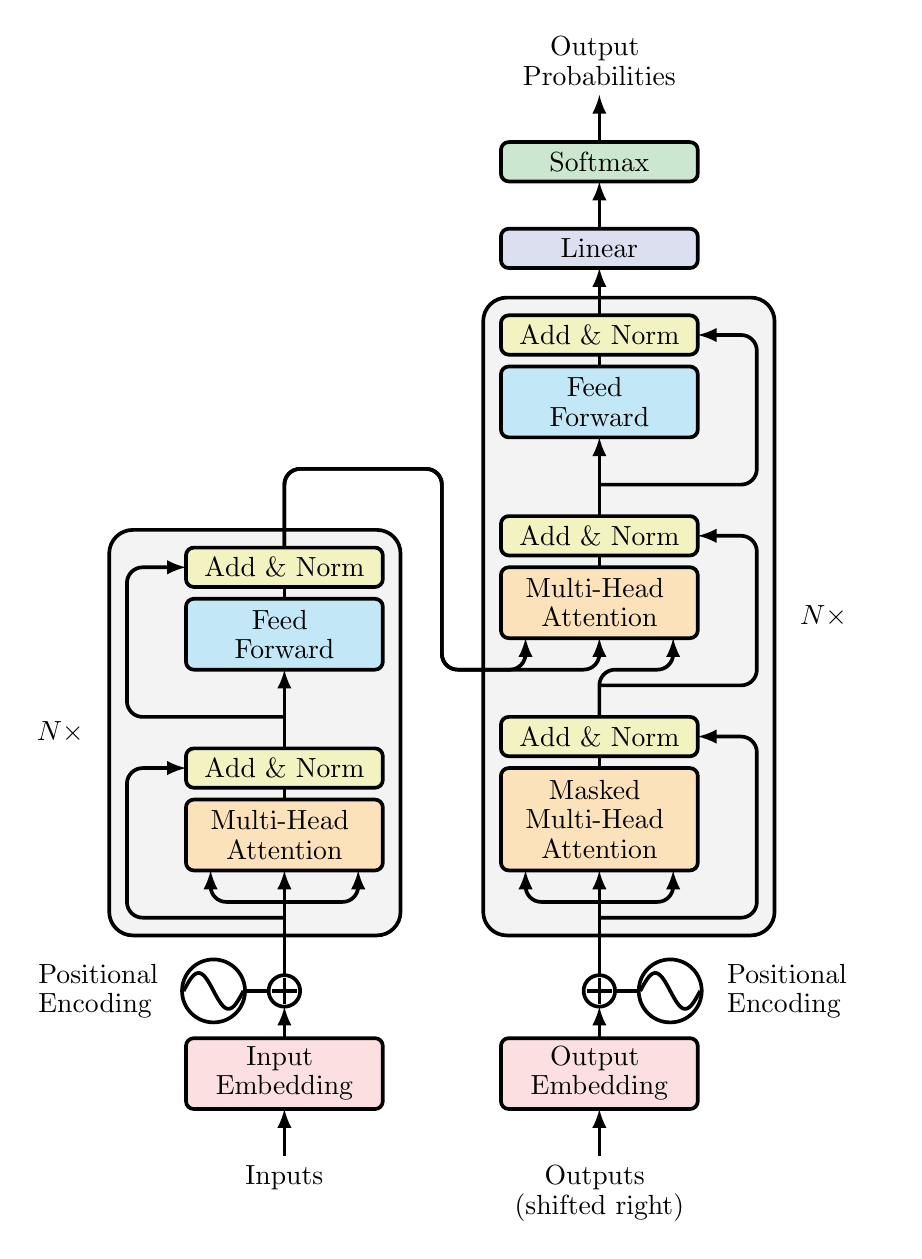
\begin{tikzpicture}
  \definecolor{emb_color}{RGB}{252,224,225}
  \definecolor{multi_head_attention_color}{RGB}{252,226,187}
  \definecolor{add_norm_color}{RGB}{242,243,193}
  \definecolor{ff_color}{RGB}{194,232,247}
  \definecolor{softmax_color}{RGB}{203,231,207}
  \definecolor{linear_color}{RGB}{220,223,240}
  \definecolor{gray_bbox_color}{RGB}{243,243,244}
  \draw[fill=gray_bbox_color, line width=0.046875cm, rounded corners=0.300000cm] (-0.975000, 6.455000) -- (2.725000, 6.455000) -- (2.725000, 1.305000) -- (-0.975000, 1.305000) -- cycle;
  \draw[fill=gray_bbox_color, line width=0.046875cm, rounded corners=0.300000cm] (3.775000, 9.405000) -- (7.475000, 9.405000) -- (7.475000, 1.305000) -- (3.775000, 1.305000) -- cycle;
  \draw[line width=0.046875cm, fill=emb_color, rounded corners=0.100000cm] (0.000000, 0.000000) -- (2.500000, 0.000000) -- (2.500000, -0.900000) -- (0.000000, -0.900000) -- cycle;
  \node[text width=2.500000cm, align=center] at (1.250000,-0.450000) {Input \vspace{-0.05cm} \linebreak Embedding};
  \draw[line width=0.046875cm, fill=emb_color, rounded corners=0.100000cm] (4.000000, 0.000000) -- (6.500000, 0.000000) -- (6.500000, -0.900000) -- (4.000000, -0.900000) -- cycle;
  \node[text width=2.500000cm, align=center] at (5.250000,-0.450000) {Output \vspace{-0.05cm} \linebreak Embedding};
  \draw[line width=0.046875cm, fill=add_norm_color, rounded corners=0.100000cm] (0.000000, 3.680000) -- (2.500000, 3.680000) -- (2.500000, 3.180000) -- (0.000000, 3.180000) -- cycle;
  \node[text width=2.500000cm, align=center] at (1.250000,3.430000) {Add \& Norm};
  \draw[line width=0.046875cm, fill=multi_head_attention_color, rounded corners=0.100000cm] (0.000000, 3.030000) -- (2.500000, 3.030000) -- (2.500000, 2.130000) -- (0.000000, 2.130000) -- cycle;
  \node[text width=2.500000cm, align=center] at (1.250000,2.580000) {Multi-Head \vspace{-0.05cm} \linebreak Attention};
  \draw[line width=0.046875cm] (1.250000, 3.030000) -- (1.250000, 3.180000);
  \draw[line width=0.046875cm, fill=add_norm_color, rounded corners=0.100000cm] (4.000000, 6.630000) -- (6.500000, 6.630000) -- (6.500000, 6.130000) -- (4.000000, 6.130000) -- cycle;
  \node[text width=2.500000cm, align=center] at (5.250000,6.380000) {Add \& Norm};
  \draw[line width=0.046875cm, fill=multi_head_attention_color, rounded corners=0.100000cm] (4.000000, 5.980000) -- (6.500000, 5.980000) -- (6.500000, 5.080000) -- (4.000000, 5.080000) -- cycle;
  \node[text width=2.500000cm, align=center] at (5.250000,5.530000) {Multi-Head \vspace{-0.05cm} \linebreak Attention};
  \draw[line width=0.046875cm] (5.250000, 5.980000) -- (5.250000, 6.130000);
  \draw[line width=0.046875cm, fill=add_norm_color, rounded corners=0.100000cm] (4.000000, 4.080000) -- (6.500000, 4.080000) -- (6.500000, 3.580000) -- (4.000000, 3.580000) -- cycle;
  \node[text width=2.500000cm, align=center] at (5.250000,3.830000) {Add \& Norm};
  \draw[line width=0.046875cm, fill=multi_head_attention_color, rounded corners=0.100000cm] (4.000000, 3.430000) -- (6.500000, 3.430000) -- (6.500000, 2.130000) -- (4.000000, 2.130000) -- cycle;
  \node[text width=2.500000cm, align=center] at (5.250000,2.780000) {Masked \vspace{-0.05cm} \linebreak Multi-Head \vspace{-0.05cm} \linebreak Attention};
  \draw[line width=0.046875cm] (5.250000, 3.430000) -- (5.250000, 3.580000);
  \draw[line width=0.046875cm, fill=add_norm_color, rounded corners=0.100000cm] (0.000000, 6.230000) -- (2.500000, 6.230000) -- (2.500000, 5.730000) -- (0.000000, 5.730000) -- cycle;
  \node[text width=2.500000cm, align=center] at (1.250000,5.980000) {Add \& Norm};
  \draw[line width=0.046875cm, fill=ff_color, rounded corners=0.100000cm] (0.000000, 5.580000) -- (2.500000, 5.580000) -- (2.500000, 4.680000) -- (0.000000, 4.680000) -- cycle;
  \node[text width=2.500000cm, align=center] at (1.250000,5.130000) {Feed \vspace{-0.05cm} \linebreak Forward};
  \draw[line width=0.046875cm] (1.250000, 5.580000) -- (1.250000, 5.730000);
  \draw[line width=0.046875cm, fill=add_norm_color, rounded corners=0.100000cm] (4.000000, 9.180000) -- (6.500000, 9.180000) -- (6.500000, 8.680000) -- (4.000000, 8.680000) -- cycle;
  \node[text width=2.500000cm, align=center] at (5.250000,8.930000) {Add \& Norm};
  \draw[line width=0.046875cm, fill=ff_color, rounded corners=0.100000cm] (4.000000, 8.530000) -- (6.500000, 8.530000) -- (6.500000, 7.630000) -- (4.000000, 7.630000) -- cycle;
  \node[text width=2.500000cm, align=center] at (5.250000,8.080000) {Feed \vspace{-0.05cm} \linebreak Forward};
  \draw[line width=0.046875cm] (5.250000, 8.530000) -- (5.250000, 8.680000);
  \draw[line width=0.046875cm, fill=linear_color, rounded corners=0.100000cm] (4.000000, 10.280000) -- (6.500000, 10.280000) -- (6.500000, 9.780000) -- (4.000000, 9.780000) -- cycle;
  \node[text width=2.500000cm, align=center] at (5.250000,10.030000) {Linear};
  \draw[line width=0.046875cm, fill=softmax_color, rounded corners=0.100000cm] (4.000000, 11.380000) -- (6.500000, 11.380000) -- (6.500000, 10.880000) -- (4.000000, 10.880000) -- cycle;
  \node[text width=2.500000cm, align=center] at (5.250000,11.130000) {Softmax};
  \draw[line width=0.046875cm] (1.250000, 0.600000) circle (0.200000);
  \draw[line width=0.046875cm] (1.410000, 0.600000) -- (1.090000, 0.600000);
  \draw[line width=0.046875cm] (1.250000, 0.760000) -- (1.250000, 0.440000);
  \draw[line width=0.046875cm] (5.250000, 0.600000) circle (0.200000);
  \draw[line width=0.046875cm] (5.410000, 0.600000) -- (5.090000, 0.600000);
  \draw[line width=0.046875cm] (5.250000, 0.760000) -- (5.250000, 0.440000);
  \draw[line width=0.046875cm] (0.350000, 0.600000) circle (0.400000);
  \draw[line width=0.046875cm] (-0.030000, 0.600000) -- (-0.014490, 0.629156) -- (0.001020, 0.657833) -- (0.016531, 0.685561) -- (0.032041, 0.711884) -- (0.047551, 0.736369) -- (0.063061, 0.758616) -- (0.078571, 0.778258) -- (0.094082, 0.794973) -- (0.109592, 0.808486) -- (0.125102, 0.818576) -- (0.140612, 0.825077) -- (0.156122, 0.827883) -- (0.171633, 0.826946) -- (0.187143, 0.822284) -- (0.202653, 0.813971) -- (0.218163, 0.802145) -- (0.233673, 0.786999) -- (0.249184, 0.768783) -- (0.264694, 0.747796) -- (0.280204, 0.724382) -- (0.295714, 0.698925) -- (0.311224, 0.671845) -- (0.326735, 0.643584) -- (0.342245, 0.614608) -- (0.357755, 0.585392) -- (0.373265, 0.556416) -- (0.388776, 0.528155) -- (0.404286, 0.501075) -- (0.419796, 0.475618) -- (0.435306, 0.452204) -- (0.450816, 0.431217) -- (0.466327, 0.413001) -- (0.481837, 0.397855) -- (0.497347, 0.386029) -- (0.512857, 0.377716) -- (0.528367, 0.373054) -- (0.543878, 0.372117) -- (0.559388, 0.374923) -- (0.574898, 0.381424) -- (0.590408, 0.391514) -- (0.605918, 0.405027) -- (0.621429, 0.421742) -- (0.636939, 0.441384) -- (0.652449, 0.463631) -- (0.667959, 0.488116) -- (0.683469, 0.514439) -- (0.698980, 0.542167) -- (0.714490, 0.570844) -- (0.730000, 0.600000);
  \draw[line width=0.046875cm] (6.150000, 0.600000) circle (0.400000);
  \draw[line width=0.046875cm] (5.770000, 0.600000) -- (5.785510, 0.629156) -- (5.801020, 0.657833) -- (5.816531, 0.685561) -- (5.832041, 0.711884) -- (5.847551, 0.736369) -- (5.863061, 0.758616) -- (5.878571, 0.778258) -- (5.894082, 0.794973) -- (5.909592, 0.808486) -- (5.925102, 0.818576) -- (5.940612, 0.825077) -- (5.956122, 0.827883) -- (5.971633, 0.826946) -- (5.987143, 0.822284) -- (6.002653, 0.813971) -- (6.018163, 0.802145) -- (6.033673, 0.786999) -- (6.049184, 0.768783) -- (6.064694, 0.747796) -- (6.080204, 0.724382) -- (6.095714, 0.698925) -- (6.111224, 0.671845) -- (6.126735, 0.643584) -- (6.142245, 0.614608) -- (6.157755, 0.585392) -- (6.173265, 0.556416) -- (6.188776, 0.528155) -- (6.204286, 0.501075) -- (6.219796, 0.475618) -- (6.235306, 0.452204) -- (6.250816, 0.431217) -- (6.266327, 0.413001) -- (6.281837, 0.397855) -- (6.297347, 0.386029) -- (6.312857, 0.377716) -- (6.328367, 0.373054) -- (6.343878, 0.372117) -- (6.359388, 0.374923) -- (6.374898, 0.381424) -- (6.390408, 0.391514) -- (6.405918, 0.405027) -- (6.421429, 0.421742) -- (6.436939, 0.441384) -- (6.452449, 0.463631) -- (6.467959, 0.488116) -- (6.483469, 0.514439) -- (6.498980, 0.542167) -- (6.514490, 0.570844) -- (6.530000, 0.600000);
  \draw[line width=0.046875cm, -latex] (1.250000, 3.680000) -- (1.250000, 4.680000);
  \draw[line width=0.046875cm, -latex] (5.250000, 6.630000) -- (5.250000, 7.630000);
  \draw[line width=0.046875cm, -latex] (5.250000, 9.180000) -- (5.250000, 9.780000);
  \draw[line width=0.046875cm, -latex] (5.250000, 10.280000) -- (5.250000, 10.880000);
  \draw[line width=0.046875cm, -latex] (1.250000, 0.000000) -- (1.250000, 0.400000);
  \draw[line width=0.046875cm, -latex] (1.250000, 0.800000) -- (1.250000, 2.130000);
  \draw[line width=0.046875cm, -latex] (5.250000, 0.800000) -- (5.250000, 2.130000);
  \draw[line width=0.046875cm, -latex] (5.250000, 0.000000) -- (5.250000, 0.400000);
  \draw[line width=0.046875cm] (0.750000, 0.600000) -- (1.050000, 0.600000);
  \draw[line width=0.046875cm] (5.450000, 0.600000) -- (5.750000, 0.600000);
  \draw[-latex, line width=0.046875cm, rounded corners=0.200000cm] (1.250000, 4.080000) -- (-0.750000, 4.080000) -- (-0.750000, 5.980000) -- (0.000000, 5.980000);
  \draw[-latex, line width=0.046875cm, rounded corners=0.200000cm] (1.250000, 1.530000) -- (-0.750000, 1.530000) -- (-0.750000, 3.430000) -- (0.000000, 3.430000);
  \draw[-latex, line width=0.046875cm, rounded corners=0.200000cm] (5.250000, 1.530000) -- (7.250000, 1.530000) -- (7.250000, 3.830000) -- (6.500000, 3.830000);
  \draw[-latex, line width=0.046875cm, rounded corners=0.200000cm] (5.250000, 4.480000) -- (7.250000, 4.480000) -- (7.250000, 6.380000) -- (6.500000, 6.380000);
  \draw[-latex, line width=0.046875cm, rounded corners=0.200000cm] (5.250000, 7.030000) -- (7.250000, 7.030000) -- (7.250000, 8.930000) -- (6.500000, 8.930000);
  \draw[-latex, line width=0.046875cm, rounded corners=0.200000cm] (1.250000, 1.730000) -- (0.312500, 1.730000) -- (0.312500, 2.130000);
  \draw[-latex, line width=0.046875cm, rounded corners=0.200000cm] (1.250000, 1.730000) -- (2.187500, 1.730000) -- (2.187500, 2.130000);
  \draw[-latex, line width=0.046875cm, rounded corners=0.200000cm] (5.250000, 1.730000) -- (4.312500, 1.730000) -- (4.312500, 2.130000);
  \draw[-latex, line width=0.046875cm, rounded corners=0.200000cm] (5.250000, 1.730000) -- (6.187500, 1.730000) -- (6.187500, 2.130000);
  \draw[-latex, line width=0.046875cm, rounded corners=0.200000cm] (1.250000, 6.230000) -- (1.250000, 7.230000) -- (3.250000, 7.230000) -- (3.250000, 4.680000) -- (4.312500, 4.680000) -- (4.312500, 5.080000);
  \draw[-latex, line width=0.046875cm, rounded corners=0.200000cm] (1.250000, 6.230000) -- (1.250000, 7.230000) -- (3.250000, 7.230000) -- (3.250000, 4.680000) -- (5.250000, 4.680000) -- (5.250000, 5.080000);
  \draw[-latex, line width=0.046875cm, rounded corners=0.200000cm] (5.250000, 4.080000) -- (5.250000, 4.680000) -- (6.187500, 4.680000) -- (6.187500, 5.080000);
  \draw[line width=0.046875cm, -latex] (1.250000, -1.500000) -- (1.250000, -0.900000);
  \draw[line width=0.046875cm, -latex] (5.250000, -1.500000) -- (5.250000, -0.900000);
  \draw[line width=0.046875cm, -latex] (5.250000, 11.380000) -- (5.250000, 11.980000);
  \node[text width=2.500000cm, anchor=north, align=center] at (1.250000,-1.500000) {Inputs};
  \node[text width=2.500000cm, anchor=north, align=center] at (5.250000,-1.500000) {Outputs \vspace{-0.05cm} \linebreak (shifted right)};
  \node[text width=2.500000cm, anchor=south, align=center] at (5.250000,11.980000) {Output \vspace{-0.05cm} \linebreak Probabilities};
  \node[anchor=east] at (-1.175000,3.880000) {$N\times$};
  \node[anchor=west] at (7.675000,5.355000) {$N\times$};
  \node[text width=2.000000cm, anchor=east] at (0.250000,0.600000) {Positional \vspace{-0.05cm} \linebreak Encoding};
  \node[text width=2.000000cm, anchor=west] at (6.750000,0.600000) {Positional \vspace{-0.05cm} \linebreak Encoding};
\end{tikzpicture}
    }
  \end{center}
  \caption{The transformer architecture as presented by \citet{NIPS2017_3f5ee243}. It consists of an encoder (left) and a decoder (right). Both the encoder and the decoder consist of layers, which are displayed as blocks in the illustration. These layers are repeated multiple times, allowing the model to process more complex information.}%
  \label{fig:transformerArchitecture}
\end{figure}

\section{Steering of Large Language Models}
\label{sec:background:llm:steering}

Although \acp{llm} are highly effective at generating coherent and fluent text, it is often desirable to guide the generated text to follow specific constraints or stylistic forms. It is also essential to prevent models from generating toxic or inappropriate content. Several steering methods have been developed to address these challenges.

One widely used method is \textbf{prompt engineering}, which involves steering the model by modifying the input prompt provided during inference. The key advantage of this approach is that it does not require any model training (\cite{schulhoffPromptReportSystematic2024}).

There are several variations of prompt engineering. One important type involves changing the system prompt, which is particularly relevant in chat-based \acp{llm}. A system prompt defines how a model behaves and what tone it uses throughout a conversation. Although it is hidden from the user, the system prompt can influence the model to adopt a specific persona, adhere to formatting rules, or follow safety guidelines. For instance, the system prompt can instruct the model to act as a helpful tutor or avoid discussing certain topics. This steering technique will be evaluated in this thesis.

Another variant of prompt engineering is few-shot prompting. With this approach, the prompt contains instructions for the task and a few examples of correct task completions. These examples allow the model to generalize to similar tasks by recognizing patterns.

% chain-of-thought prompting by Wei et al., 2022 % TODO: include this?

\textbf{Fine-tuning} is a more resource-intensive method of steering that involves updating the parameters of the model using task-specific data. Although fine-tuning can yield strong performance, it is often too expensive for \acp{llm} due to their size. Furthermore, using a different fine-tuned model for each task can be inefficient and impractical.

To mitigate these issues, parameter-efficient fine-tuning methods have been developed. These methods freeze the pre-trained model weights and only train a small number of additional parameters. One such method is prefix tuning (\cite{liPrefixtuningOptimizingContinuous2021}), where a learned vector (prefix) is prepended to the model input. This method achieves competitive performance while training only \SI{0.1}{\percent} of the model's parameters. Another example is LoRA (\cite{huLoRALowrankAdaptation2021}), which introduces trainable low-rank matrices into the model while keeping the original weights fixed. LoRA reduces the number of trainable parameters by a factor of \num{10000} without compromising performance.

% \textbf{Reinforcement Learning from Human Feedback (RLHF)} % TODO: include this?

A recent alternative to these methods is \textbf{activation steering}, which directly alters the hidden states of an \acs{llm} during inference to guide its output. These hidden states are generally accessed at the end of each transformer layer. Modern \acp{llm} typically consist of between \num{20} and \num{100} such layers, with deeper layers typically encoding more abstract and sophisticated concepts (\cite{bogdanEmergentEffectsScaling2025}).

Activation steering involves identifying and extracting the hidden states that correspond to specific concepts in a single forward pass. These extracted vectors, known as steering vectors, are added to the internal states of the model during inference to guide the generation process in the desired direction (\cite{konenStyleVectorsSteering2024,turnerActivationAdditionSteering2024,subramaniExtractingLatentSteering2022}).

\clearpage

\chapter{Datasets}%
\label{sec:datasets}

% TODO: introduction

\section{Stack Exchange Dataset}%
\label{sec:datasets:stackex}
The main dataset used in this thesis is derived from Stack Exchange\footnote{\url{https://stackexchange.com/}}, a network of online Q\&A forums. Stack Exchange is structured as a collection of topic-specific communities where users can post questions and provide answers. For this thesis, the focus is on forums for specific groups, such as \url{biology.stackexchange.com}, designed for biologists and others interested in biology-related discussions.

To ensure that the answers that are being used for the thesis actually include explanations, only questions that begin with \enquote{what}, \enquote{how}, or \enquote{why} are selected, as these typically elicit detailed conceptual explanations in the answers according to \citet{millerExplanationArtificialIntelligence2019}. From the full set of Stack Exchange forums, \num{16} group-specific forums are identified as relevant. % TODO: why 11?
Out of these, \num{11} are selected for the experimental evaluation carried out in this thesis. The specific groups and the corresponding number of answers used from each are documented in Appendix~\ref{sec:appendix:datasets:stackex}.
% To ensure the answers used in the thesis include explanations, only questions beginning with \enquote{what}, \enquote{how}, or \enquote{why} are selected, as these typically elicit detailed, conceptual responses. Of the full set of Stack Exchange forums, \num{16} group-specific forums were identified as relevant. \num{11} of these are selected for the experimental evaluation carried out in this thesis. The specific groups and the number of answers used from each are documented in Appendix~\ref{sec:appendix:datasets:stackex}.

\section{AskX Dataset}%
\label{sec:datasets:askx}
The second dataset used in this thesis is derived from Reddit\footnote{\url{https://www.reddit.com/}}, a widely used online discussion platform where users submit posts and others respond. Reddit is organized into subforums, known as \enquote{subreddits}, that focus on specific topics and have their own rules and moderation policies.

This dataset focuses on a specific category of subreddits that follow the \enquote{AskX} schema. In these subreddits, any user may pose a question, but only individuals belonging to a specific demographic are expected to respond. Examples include \enquote{Askelectricians}, where only electricians are encouraged to answer, and \enquote{Askteens}, where answers should come from teenagers. A total of \num{26} such AskX subreddits were initially identified.

% TODO: is this the correct number?
From this pool, \num{24} subreddits are manually selected and grouped to create a unified corpus. The grouping process is necessary because some subreddits do not have enough answers to be treated independently. As with the Stack Exchange dataset, only questions that start with \enquote{what}, \enquote{how}, or \enquote{why} are retained to ensure that the dataset contains genuine explanations. Further details on the selected subreddits and the grouping process are provided in Appendix~\ref{sec:appendix:datasets:askx}.

\section{Steering Dataset}%
\label{sec:datasets:steering}
For steering experiments, it is essential to use high-quality questions that elicit meaningful, conceptually rich responses. While questions from the Stack Exchange and AskX datasets could be used for this purpose, they do not consistently meet the quality and clarity required for steering tasks.

% TODO: from kilt, I used ELI5 test dataset
Instead, this thesis uses a steering dataset consisting of questions taken from the works of \citet{petroni-etal-2021-kilt,rooeinKnowYourAudience2023}. These studies focus on question answering and compile carefully curated lists of what, how, and why questions. These questions are particularly well-suited to the steering experiments conducted in this thesis and offer a reliable benchmark for evaluating the ability of the model to generate group-specific responses. Further details regarding this dataset can be found in Appendix~\ref{sec:appendix:datasets}.

\clearpage

% !TeX root = ..\..\thesis.tex
\chapter{Approach}
\label{sec:approach}


\section{Data Collection}
\label{sec:approach:dataCollection}


\section{Architecture and Models used}
\label{sec:approach:architectureModels}

\subsection{Architecture}
\label{sec:approach:architectureModels:architecture}

\begin{itemize}
  \item Style Sentence Generation
  \item Clustering
  \item Selection of Style Vector Attributes
  \item Training SFAM and LISA
  \item Training the embedding model
  \item Prompt Steering
  \item Activation Steering
\end{itemize}

\subsection{Models}
\label{sec:approach:architectureModels:models}

\begin{itemize}
  \item Llama3.2
  \item Sentence Transformer
  \item DeBERTaV3
  \item \ldots
\end{itemize}


\section{Evaluation Metrics}
\label{sec:approach:evaluationMetrics}

\begin{itemize}
  \item SFAM
        \begin{itemize}
          \item accuracy and F1 with regard to labels from select examples of the style sentence generation (was the sentence used or not)
        \end{itemize}
  \item LISA
        \begin{itemize}
          \item MSE, MAE, avg. cosine similarity compared to SFAM prediction
          \item accuracy and F1 compared to SFAM where both predictions are rounded
        \end{itemize}
  \item embedding model
        \begin{itemize}
          \item accuracy through triplet loss
                %? \item variance inside groups
        \end{itemize}
  \item steering methods
        \begin{itemize}
          \item improvement of L2 distance to group median compared to embedding of unsteered generation
                \begin{itemize}
                  \item how strong is the steering?
                \end{itemize}
          \item cosine similarity between the vector that is the difference between embedding of steered and unsteered generation
                \begin{itemize}
                  \item is the steering in the correct direction?
                \end{itemize}
                %? \item the absolute times that the resulting group is the correct one (according to the embedding)
        \end{itemize}
\end{itemize}


\section{Style Sentence Generation}
\label{sec:approach:styleSentenceGeneration}

The style sentences that form the dimensions of the interpretable style vector are generated by prompting a \acl{llm} in a two-step procedure.

For step one, the \ac{llm} is presented with a zero-shot prompt to produce a description of the text. This step is repeated 92 times, each time with a different prompt that focuses on a specific aspect of the text. 6 prompts are relatively open and only give a loose direction on which style should be described by the model. 84 prompts are targeted towards an explicit stylistic feature. These prompts follow the work of \citet{patelLearningInterpretableStyle2023,tausczikPsychologicalMeaningWords2010} to get the model to focus on a broad variety of style that is important for the study of language.

In addition to these prompts aimed at stylistic features, there are two prompts which are focusing on the knowledge and experience of the author. While the background knowledge of the author is not as important for the group membership detection as the style of the text, it is helpful information for the steering task that is covered in later sections.

After generating the style descriptions, the \ac{llm} is prompted a second time to rewrite the description as a list of sentences. The model is instructed to write each sentence in a consistent form like \enquote{The author is \ldots} or \enquote{The author uses \ldots}.

Furthermore, the model is instructed to avoid negations and examples since these both lead to increasing problems with the clustering process that is described in Section~\ref{sec:approach:clustering}.
Sentences that include examples are potentially problematic because it increases the likelihood of sentences which have the exact same content while being of different shape. % TODO: better wording
Two sentences which differ only in the example are \enquote{The author uses filler words} and \enquote{The author uses filler words such as 'and', 'or' and 'furthermore'}. While this problem will be reduced by clustering similar sentences, this procedure is not perfect and will be more robust if the model avoids sentences with examples.

Negations on the other hand lead to the problem where the shape of the sentences will be too close while the content is very different. There is a high chance that the sentences \enquote{The author does use long sentences} and \enquote{The author does not use long sentences} will be clustered together because so much of them is the same even though they state the opposite of each other.
Additionally, the dimensions of the final style vector should not include any negated attributes since the expression \enquote{The author uses short sentences} is much clearer than \enquote{The author does not use long sentences}.

Since the model might produce sentences with negations or examples despite the prompt, each of the generated sentences is checked automatically.

Per description, each distinct style sentence is recorded only once, even if the model generates it multiple times. This is done in case the model generates a bad answer where one sentence is repeated many times.

The whole process can be seen in Figure~\ref{fig:styleSentenceGeneration}.

\begin{figure}[ht]
  \newlength{\mytw}
\settowidth{\mytw}{A few lines of text in a block}
\begin{center}
  \begin{tikzpicture}
    [> = latex', auto,
      block/.style ={
          rectangle,
          draw=black,
          thick,
          % align=flush center,
          rounded corners,
          % minimum height=4em
        },
    ]
    \node[block, text width=0.7\linewidth] (answer) {\textbf{Input Text:}\\If the judge believes the award is too high or too low, the judge can use additur or remittitur to reduce the damages. These are essentially offers to both parties to agree to the change in damages. If both parties do not agree, the court can order a new trial.};

    \node[block, minimum height=3cm, text width=0.4\linewidth, below left=of answer.south] (prompt1) {\textbf{Prompt 1 (Grammar Style):}\\Write a long paragraph describing the unique grammar style of the following passage without referring to specifics about the topic.};
    \node[align=flush center, minimum height=3cm, text width=0.2\linewidth, below=1cm of answer.south] (prompt2) {\ldots};
    \node[block, minimum height=3cm, text width=0.4\linewidth, below right=of answer.south] (prompt3) {\textbf{Prompt 92 (Background Knowledge):}\\Write a description of the background knowledge the author has based on the following passage.};

    \draw[->] (answer.south) -- (prompt1.north);
    \draw[->] (answer.south) -- (prompt2.north);
    \draw[->] (answer.south) -- (prompt3.north);

    \node[block, align=flush center, minimum height=1cm, text width=0.4\linewidth, below=1cm of prompt1] (description1) {Style Description};
    \node[align=flush center, minimum height=1cm, text width=0.2\linewidth, below=1cm of prompt2] (description2) {\ldots};
    \node[block, align=flush center, minimum height=1cm, text width=0.4\linewidth, below=1cm of prompt3] (description3) {Style Description};

    \draw[->] (prompt1.south) -- (description1.north);
    \draw[->] (prompt2.south) -- (description2.north);
    \draw[->] (prompt3.south) -- (description3.north);

    \node[block, text width=0.95\linewidth, below=1cm of description2] (sentence_prompt) {\textbf{Prompt:}\\Rewrite this description as a long list of short sentences describing the author's writing style  where each sentence is in the format of \enquote{The author is X.} or \enquote{The author uses X.}.};

    \draw[->] (description1.south) -- ++(0,-1cm);
    \draw[->] (description2.south) -- ++(0,-1cm);
    \draw[->] (description3.south) -- ++(0,-1cm);

    \node[block, text width=0.95\linewidth, below=1cm of sentence_prompt] (attributes) {\textbf{Style Attributes:}\\
      % The author uses the passive voice. \\
      % The author uses active voice. \\
      % The author uses sentence fragments. \\
      % The author uses run-on sentences. \\
      % The author uses words related to visual perception. \\
      % The author uses words expressing wellness. \\
      % The author uses a neutral tone. \\
      The author uses words related to risk. \\
      The author uses words related to allure. \\
      The author uses words indicating poverty. \\
      The author uses words expressing needs. \\
      The author uses numbers. \\
      The author explains legal concepts. \\
      The author uses words indicating men. \\
      The author uses the word judge. \\
      \ldots
    };

    \draw[->] (sentence_prompt.south) -- +(0,-1cm);
    \draw[->] let \p1 = (sentence_prompt.south), \p2 = (description1) in (\x2,\y1) -- +(0,-1cm);
    \draw[->] let \p1 = (sentence_prompt.south), \p2 = (description3) in (\x2,\y1) -- +(0,-1cm);
  \end{tikzpicture}
\end{center}

  % TODO: better caption
  \caption{The process to generate style sentences.}
  \label{fig:styleSentenceGeneration}
\end{figure}


\section{Clustering}
\label{sec:approach:clustering}
A strength of the method to create style sentences described in Section~\ref{sec:approach:styleSentenceGeneration} is the lack of constraints which results in a large variety of generated sentences. However, this leads to the problem that sentences with the same content can have many different forms. An example for this would be the sentences \enquote{The author uses short and concise sentences.} and \enquote{The author uses concise and short sentences.}, which have exactly the same meaning while having a distinct form.

Since the approach up to this point only checked if sentences are exactly identical, it is more difficult to compare different input texts and to find texts that are an example of a specific style sentence. Additionally, it could be that a sentence would be a good attribute for the style sentence but is not selected by the algorithm described in Section~\ref{sec:approach:selection} because it is used with many different variations.
To solve this problem, my approach includes clustering the sentences by the cosine similarity of their embeddings with a sentence embedding model. % TODO: citation for the model (and name?)

The clustering algorithm first computes a radius neighbor graph of all sentences where sentences which have a cosine similarity of more than \num{\minCosineSimilarity}. Subsequently, the clusters are sorted by size and all sentences that have been included in a larger cluster are deleted from all smaller clusters to ensure that each sentence is only included in one cluster. At the same time, it has to be ensured that no sentence is left out of every cluster because for further approaches, the clusters are the relevant data.

For the resulting clusters, the style sentence that is closest to the center is the representative sentence of the whole cluster.

The size of the resulting synthetic dataset after clustering can be found in table~\ref{table:syntheticDataset}.

\begin{table}
  \begin{center}
    % TODO: alignment of numbers inside the \num command
    \begin{tabular}{lS}
      \toprule
                   & {Number of data points} \\ \midrule
      Answers      & \numAnswersStyleVector  \\
      Prompts      & \numPrompts             \\
      Descriptions & \numStyleDescriptions   \\
      Sentences    & \numStyleSentences      \\
      Clusters     & \numClusters            \\ \bottomrule
    \end{tabular}
    \caption{The number of answers and prompts used to create the synthetic dataset and the size of the resulting dataset.}
    \label{table:syntheticDataset}
  \end{center}
\end{table}


% \begin{itemize}
%   \item often, style sentences are generated that are very similar
%   \item e.g. \enquote{The author uses short and concise sentences.} and \enquote{The author uses concise and short sentences.}
%   \item If one style sentence is used very often but in many different variations, it may not get selected for the style sentence vector because each variation by itself has not occured often enough
%   \item The sentences are embedded with the model x % TODO: write that here?
%   \item because of that, all style sentences are clustered so that sentences which embeddings have a cosine distance of less than 0.15 count as the same sentence. The sentence that is closest to the center functions as the representation of the whole cluster
%   \item each sentence can only be in one cluster; if it is in multiple clusters it is removed from all but the largest
%   \item each sentence has to be in exactly one clusters, so many clusters include only one sentence
% \end{itemize}


\section{Selecting the Style Vector Attributes}
\label{sec:approach:selection}

Following the previous steps, there is now a synthetic dataset with \num{\numClusters} that describe \num{\numAnswersStyleVector} answers by \num{\numGroups}. Since the final style vector will only consist of \num{\styleVectorSize} attributes, a process to select the best attributes is needed. This selection is carried out in multiple steps.

\subsection{Selection of target attributes}
\label{sec:approach:selection:targetAttributes}
Following the work of \citet{patelLearningInterpretableStyle2023}, the first \num{\numTargetPrompts} attributes of the style vector will be selected to correspond to the \num{\numTargetPrompts} target prompts which were described in section~\ref{sec:approach:styleSentenceGeneration}.
This is done to ensure that the style vector has a robust foundation on some features that are manually selected for being relevant for stylistic research. The ability to automatically create most of the style vector is not reduced since the target attributes only account for around \SI{10}{\percent} of its size.

These attributes are found by creating sentences of the form \enquote{The author uses <target>} and embedding using the SentenceTransformer Model. % TODO: correct name
Afterward, for each sentence the style cluster with the highest cosine similarity is found.
All clusters that have been chosen this way to represent the
% TODO: find a nice final sentence


\subsection{Step 2}
% \label{} TODO:
An important characteristic of all attributes that are part of the style vector is that they are as meaningful as possible and helpful to distinguish different groups. Because of that, this step in the cluster selection ensures that only clusters which are used to describe texts by less than \clusterMaxGroupRatio{} of the groups are selected. The cutoff ratio of groups follows the work of \citet{patelLearningInterpretableStyle2023}.

For the next steps of the cluster selection, it is also important that there are not too many possible clusters to select from, otherwise the computation would need too much time and memory. To quickly reduce the number of clusters, the number of times the cluster was used to describe answers is taken into account. The required number of times used is increased until the resulting number of clusters is smaller than \num{\maxClustersFirstSelection}. This number was chosen to be small enough for the following computation but big enough to enable a meaningful selection of style vector attributes.

% TODO: include this?
A cluster could be used multiple times to describe the same answer. Although the sentence produced by each prompt is only counted once per prompt, multiple prompts could use the same or similar enough sentences to describe the answer. For this selection however, only the number of answers that have been described with the cluster are being counted and not how often the cluster was being used.

\subsection{Step 3}
% \label{} TODO:
To ensure that the style vector covers a wide range of attributes, it is important that the attributes do not cover too similar topics. This selection step fulfills this requirement by ensuring that the style vector attributes have a maximum cosine similarity of \num{\maxCosineSimilarity}. This process works by ordering the clusters by occurrence, selecting them one after the other and deleting all clusters that are too close to the ones that have already been selected.

In the work of \citeauthor{patelLearningInterpretableStyle2023}, they use a maximum cosine similarity of \num{0.8} as a cutoff. I decided to use a lower maximum similarity to increase the variance of the style vector attribute and because of the clusters. % TODO: better explanation

\subsection{Step 4}
% \label{} TODO:
The first \num{\numTargetPrompts} attributes of the style vector are the target attributes that were selection in Section~\ref{sec:approach:selection:targetAttributes}. The next \num{\minNumKnowledgePrompts} attributes are knowledge clusters, that is clusters of sentences that were produced by knowledge prompts. The rest of the style attributes are selected in this step to be the ones with the highest range of accordance. % TODO: better word than accordance?

Range of accordance means that the range between the answers that match the attribute really well and the ones that do not match is as big as possible. This further increases the probability that the attributes are well suited to distinguish between different answers and groups.

First of all, the similarity between all clusters that remain after the first selection steps are computed. Afterwards, the for each cluster and each answer the average similarity to all other clusters that have been used to describe that answer is computed. TODO:


% \begin{itemize}
%   \item \minNumKnowledgePrompts{} knowledge clusters are selected
%   \item compute similarities between clusters selected at this stage
%   \item for all clusters, compute the average similarity of all input texts by looking at the clusters that have been used to describe that input text
%   \item sort the clusters by the difference between the most and least matching input text
%   \item select the clusters with the highest difference
%   \item this is done because a style attribute will probably hold more meaningful information and is better suited to differentiate texts if it is very similar to some and very dissimilar to other texts
% \end{itemize}


\section{Training and Testing \acs{sfam}}
\label{sec:approach:sfam}

The goal of the method presented in this thesis is to create interpretable style vectors with values between \num{0} and \num{1} that correspond to real world values. To create these values, I will train a model that follows the \acf{sfam} that was presented by \citet{patelLearningInterpretableStyle2023}. It takes an attribute sentence and a text and outputs and agreement score that corresponds to how well the attribute sentence fits to the text.

\ac{sfam} is trained on the synthetic dataset which was created in earlier steps as described in Section~\ref{sec:approach:styleSentenceGeneration}. The training data includes the unclustered knowledge and style sentences and the input texts that were described by them. There is however some preprocessing necessary, because just because an attribute sentence was not used to describe a text does not mean the text does not match the sentence. It could be that the text was described by a similar sentence or that the \ac{llm} just skipped a topic when describing one text.

The attribute sentences that are used for training are selected in a process similar to the one described in Section%~\ref{}. TODO:
First, the similarity between all attribute sentences and all Attribute Vector dimensions are computed. Then, for each sentence and each text the average similarity to the dimensions that were used to describe the text is computed. The texts are then sorted by their similarity to the attribute sentence. If the sentence has been used to describe one of the \SI{1}{\percent} most similar texts, this text will be used as a positive training sample and the most dissimilar text where the sentence was not used to describe it is used as a negative training sample. Otherwise, the sentence will not be used for training.

The result dataset is balanced regarding positive and negative samples and has a high probability to only include sentences which actually fit the texts. % TODO: write better
The same process is used to create the validation and test dataset using different answers. % TODO: write here that the style sentences are largely distinct or later in experiments?

% \begin{itemize}
%   \item \ac{sfam} is a model that takes a style sentence and a text as input and produces an agreement score
%   \item training data
%         \begin{itemize}
%           % \item the \numStyleSentences{} style sentences are used for training % do not use numbers for approach
%           \item there are distinct sets of input texts for training, validation and test datasets
%           \item these lead to mostly different sentences (also the differences may be small)
%           \item of all sentences, the best are selected
%                 \begin{itemize}
%                   \item compute similarity to all style vector attributes (which are clusters)
%                   \item for each sentence, compute the most similar and most dissimilar input text according to the average similarity to all style attributes that have been used to describe that text (like the final selection of style vector attributes, see Section~\ref{sec:approach:selection}) % TODO: is there a more specific reference to a subsection?
%                   \item if one of the ten most similar input texts was actually described by the style sentence, it is chosen as a positive training sample and the least similar input text that was not described by the sentence as a negative sample
%                   \item otherwise, the sentence is not used for training
%                   \item the same is done for validation and test
%                 \end{itemize}
%         \end{itemize}
%   \item \ac{sfam} is a finetuned DeBERTaV3 model
%         \begin{itemize}
%           \item two fully connected layers with a ReLu in between % TODO: look up
%           \item finally a sigmoid activation function to produce values between 0 and 1
%         \end{itemize}
%   \item optional hyperparameter optimization (with optuna -> citation?) to discover optimal learning rate and weight decay
%   \item early stopping callback with patience of three
%   \item validation metric of accuracy
%   \item testing metric accuracy and f1
% \end{itemize}


\section{Training and Testing \acs{lisa}}
\label{sec:approach:lisa}
While \ac{sfam} produces the Attribute Vector with exactly the values that are required, it needs on forward pass per dimension of the vector. Even with an optimized model this takes a too long time for the most applications. The solution is to train an additional model which for the \acf{lisa} model proposed by \citet{patelLearningInterpretableStyle2023}, which gets a text as an input and produces the full Attribute Vector in one forward pass.

The training, validation and test data is created by using \ac{sfam} to create the Attribute Vectors of the corresponding texts and training \ac{lisa} as a regression model.

% \begin{itemize}
%   \item to get values for a style vector, the \num{\styleVectorSize} forward passes by \ac{sfam} would take too long for most practical applications
%   \item train an additional model that creates the whole vector in one forward pass
%   \item \ac{lisa} like \ac{sfam} is a finetuned DeBERTaV3 model
%         \begin{itemize}
%           \item two fully connected layers with a ReLu in between % TODO: look up
%           \item finally a sigmoid activation function to produce values between 0 and 1
%         \end{itemize}
% \end{itemize}

\section{Embedding Model}
\label{sec:approach:embedding}



\section{Possible Improvement through Knowledge Attributes}
\label{sec:approach:knowledgeAttributes}


\section{Steering Text Generation with Simple Prompting}
\label{sec:approach:steering:simple}
\begin{figure}
  \begin{center}
    \begin{tikzpicture}[scale=2, >=stealth]
  % Define vectors
  \coordinate (O) at (0,0);
  \coordinate (A) at (2,1);
  \coordinate (B) at (3,3);
  \coordinate (C) at (2,4);

  % Draw vectors A, B, and C from the origin
  \draw[->, thick, blue] (O) -- (A) node[midway, below right=0cm and -1cm, sloped] {unsteered embedding};
  \draw[->, thick, red] (O) -- (B) node[midway, above, sloped] {steered embedding };
  \draw[->, thick, green!70!black] (O) -- (C) node[midway, above, sloped] {median group embedding};

  % Draw vector B - A from point A to point B
  \draw[->, thick, dashed, orange] (A) -- (B) node[midway, below right] {steering effect};

  % Optional: Draw axes
  \draw[->] (-0.5,0) -- (4,0) node[below right] {$x$};
  \draw[->] (0,-0.5) -- (0,4) node[above left] {$y$};
\end{tikzpicture}


    \caption{Embeddings of steered and unsteered generations}
  \end{center}
\end{figure}


\section{Steering Text Generation with Targeted Prompting}
\label{sec:approach:steering:targeted}


\section{Steering Text Generation with Activation Layer Manipulation}
\label{sec:approach:steering:actAdd}

\subsubsection{Extracting Steering Vectors}

\subsubsection{Generation Steering}
\clearpage

\chapter{Experiments and Evaluation}
\label{sec:experiments_evaluation}


\section{Environment and Hardware}
\label{sec:experiments_evaluation:environmentHardware}

\begin{itemize}
  \item node on a SLURM server cluster
        \begin{itemize}
          \item 32 CPU Cores % or 32?
          \item \SI{128}{\giga\byte} RAM % or 128?
          \item Nvidia A-100 GPU with \SI{40}{\giga\byte} RAM
        \end{itemize}
  \item Python Version
  \item sqlite Database as data storage? → show schema diagram in appendix
\end{itemize}


\section{Architecture and Models used}
\label{sec:approach:architectureModels}

\subsection{Architecture}
\label{sec:approach:architectureModels:architecture}

\begin{itemize}
  \item Attribute Sentence Generation
  \item Clustering
  \item Selection of Attribute Vector dimensions
  \item Training SFAM and LISA
  \item Training the embedding model
  \item Prompt Steering
  \item Activation Steering
\end{itemize}

\subsection{Models}
\label{sec:approach:architectureModels:models}

\begin{itemize}
  \item Llama3.2
  \item Sentence Transformer
  \item DeBERTaV3
  \item \ldots
\end{itemize}

\section{Implementation}

\subsection{Creation of the Synthetic Dataset}
\begin{itemize}
  \item to embed the attribute sentences, the model \textit{all-MiniLM-L12-v2} (\cite{reimersSentenceBERTSentenceEmbeddings2019}) has been used
  \item for clustering, sentences must have a cosine similarity of \num{\minCosineSimilarity} or less to be in the same cluster
  \item resulting dataset in Table~\ref{table:syntheticDataset}
\end{itemize}
\begin{table}[ht]
  \begin{center}
    % TODO: alignment of numbers inside the \num command
    \begin{tabular}{lS[table-format=7.0]}
      \toprule
                   & {Number of data points} \\ \midrule
      Answers      & \numAnswersStyleVector  \\
      Prompts      & \numPrompts             \\
      Descriptions & \numStyleDescriptions   \\
      Sentences    & \numStyleSentences      \\
      Clusters     & \numClusters            \\ \bottomrule
    \end{tabular}
    \caption{The number of answers and prompts used to create the synthetic dataset and the size of the resulting dataset.}
    \label{table:syntheticDataset}
  \end{center}
\end{table}

\subsection{Attribute Selection}
\begin{itemize}
  \item \num{\numClusters} clusters
  \item \num{\numAnswersStyleVector} answers by \num{\numGroups} groups
  \item select only \num{\styleVectorSize} attributes for the interpretable attribute vector
  \item filtering out too frequent
        \begin{itemize}
          \item max \clusterMaxGroupRatio{} of groups (number taken from \citet{patelLearningInterpretableStyle2023})
          \item number of clusters smaller er than \num{\maxClustersFirstSelection}. This number was chosen to be small enough for the following computation but big enough to enable a meaningful selection of attribute vector dimensions.
        \end{itemize}
  \item too similar
        \begin{itemize}
          \item \num{\maxCosineSimilarity} maximum cosine similarity
          \item In the work of \citeauthor{patelLearningInterpretableStyle2023}, they use a maximum cosine similarity of \num{0.8} as a cutoff. I decided to use a lower maximum similarity to increase the variance of the attribute vector dimensions and because of the clusters. % TODO: better explanation
        \end{itemize}
\end{itemize}

\begin{figure}
  \begin{center}
    \begin{tikzpicture}[
    % arrow tip
    >=Stealth,
    % box style
    box/.style={
        draw,
        rectangle,
        minimum width=50mm,
        minimum height=10mm,
        align=center
      },
    % dashed region style
    dashedbox/.style={
        draw,
        dashed,
        inner sep=6mm
      },
    % default distance between nodes
    node distance=8mm and 12mm
  ]

  % Top layer
  \node[box] (attrib) {Attribute Sentences};
  \node[box, below left=of attrib]  (stySent) {Style Sentences};
  \node[box, below right=of attrib] (knSent)  {Knowledge Sentences};

  % Clustering step
  \node[box, below=of $(stySent)!0.5!(knSent)$] (cluster)
  {Clustering by Cosine Similarity};

  % Resulting clusters
  \node[box, below left=of cluster]  (styCl) {Style Clusters};
  \node[box, below right=of cluster] (knCl)  {Knowledge Clusters};

  % Three sequential steps
  \node[box, below=of $(styCl)!0.5!(knCl)$] (step1)
  {used in maximum number of groups\\minimum usages};
  \node[box, below=of step1] (step2)
  {clusters with a minimum distance to each other};
  \node[box, below=of step2] (step3)
  {clusters with largest difference in agreement levels};

  % Dashed box around those three steps
  \node[dashedbox, fit=(step1)(step2)(step3)] {};

  % Final attribute-vector block
  \node[box, below=of step3] (attrVec) {
    \begin{tabular}{ccc}
      Targeted Style Attributes & Knowledge Attributes & Style Attributes
    \end{tabular}
    \\[2pt]
    \textbf{Attribute Vector}
  };

  % Arrows
  \draw[->] (attrib)  -- (stySent);
  \draw[->] (attrib)  -- (knSent);
  \draw[->] (stySent) -- (cluster);
  \draw[->] (knSent) -- (cluster);
  \draw[->] (cluster) -- (styCl);
  \draw[->] (cluster) -- (knCl);
  \draw[->] (styCl)    -- (step1);
  \draw[->] (knCl)     -- (step1);
  \draw[->] (step1)    -- (step2);
  \draw[->] (step2)    -- (step3);
  \draw[->] (step3)    -- (attrVec);
  \draw[->] (attrVec.west) .. controls +(-15mm,0) and +(-15mm,24mm) .. (stySent.west);

\end{tikzpicture}

  \end{center}
\end{figure}


\section{Evaluation Metrics}
\label{sec:approach:evaluationMetrics}

\begin{itemize}
  \item SFAM
        \begin{itemize}
          \item accuracy and F1 with regard to labels from select examples of the attribute sentence generation (was the sentence used or not)
        \end{itemize}
  \item LISA
        \begin{itemize}
          \item MSE, MAE, avg. cosine similarity compared to SFAM prediction
          \item accuracy and F1 compared to SFAM where both predictions are rounded
        \end{itemize}
  \item embedding model
        \begin{itemize}
          \item accuracy through triplet loss
                %? \item variance inside groups
        \end{itemize}
  \item steering methods
        \begin{itemize}
          \item improvement of L2 distance to group median compared to embedding of unsteered generation
                \begin{itemize}
                  \item how strong is the steering?
                \end{itemize}
          \item cosine similarity between the vector that is the difference between embedding of steered and unsteered generation
                \begin{itemize}
                  \item is the steering in the correct direction?
                \end{itemize}
                %? \item the absolute times that the resulting group is the correct one (according to the embedding)
        \end{itemize}
\end{itemize}


\begin{figure}
  \begin{center}
    \begin{tikzpicture}[scale=2, >=stealth]
  % Define vectors
  \coordinate (O) at (0,0);
  \coordinate (A) at (2,1);
  \coordinate (B) at (3,3);
  \coordinate (C) at (2,4);

  % Draw vectors A, B, and C from the origin
  \draw[->, thick, blue] (O) -- (A) node[midway, below right=0cm and -1cm, sloped] {unsteered embedding};
  \draw[->, thick, red] (O) -- (B) node[midway, above, sloped] {steered embedding };
  \draw[->, thick, green!70!black] (O) -- (C) node[midway, above, sloped] {median group embedding};

  % Draw vector B - A from point A to point B
  \draw[->, thick, dashed, orange] (A) -- (B) node[midway, below right] {steering effect};

  % Optional: Draw axes
  \draw[->] (-0.5,0) -- (4,0) node[below right] {$x$};
  \draw[->] (0,-0.5) -- (0,4) node[above left] {$y$};
\end{tikzpicture}


    \captionsetup{singlelinecheck=off}
    \caption[]{%
      All answers that are generated during steering are embedded using the \ac{lisa} model with the embedding head. For each question, the \ac{llm} is prompted without any steering to create an unsteered baseline. Then, for each group and each steering type, the model is prompted with the same question. The median group embedding is derived from the embeddings of all answers that have been used to train \ac{sfam} and \ac{lisa}.
      The quality of each steering method is measured with different metrics:
      \begin{enumerate*}
        \item \textbf{Steering Direction Correctness:} The cosine similarity between the steering effect vector and the optimal steering effect vector.
        \item \textbf{Steering Effect:} The euclidean distance of the steering effect vector.
        \item \textbf{Optimal Steering Effect:} The euclidean distace between the unsteered embedding and the median group embedding.
        \item \textbf{Possible Improvement:} The euclidean distance between the steered embedding and the median group embedding.
              % \item difference between steering effect and optimal steering effect
              % \item difference (or ratio?) between steering effect and possible steering effect
      \end{enumerate*}
    }
  \end{center}
\end{figure}

\section{Steering}
\label{sec:experiments_evaluation:steering}

\begin{itemize}
  \item questions taken from \citet{petroni-etal-2021-kilt,rooeinKnowYourAudience2023}
\end{itemize}
\clearpage

\chapter{Evaluation and Discussion}%
\label{sec:evaluation}

This chapter evaluates the methods and models introduced in this thesis and presents the results of the experiments described in Section~\ref{sec:experiments}. These results aim to answer the research questions stated in Section~\ref{sec:introduction:problemStatement}.

\section{Evaluating the Importance of Knowledge Attributes for the Interpretable Attribute Vector}%
\label{sec:evaluation:knowledgeAttributes}

As explained in Section~\ref{sec:experiments:knowledgeAttributes}, this experiment evaluates the importance of knowledge attributes, which are an extension to the style vectors proposed by this thesis. The experiment involves analyzing the \num{10}, \num{20}, and \num{50} most important attributes of the interpretable attribute vector per group. The results of this evaluation are presented in Table~\ref{table:knowledgeImportance}.

The results clearly show that knowledge attributes are not equally important across all groups. In particular, groups such as biologists, historians, and politicians do not rely significantly on knowledge attributes to differentiate themselves from other groups. However, knowledge attributes show at least some relevance for the majority of groups. Especially for the groups of game developers and software engineers the knowledge attributes are particularly important, with at least half of the ten most important attributes being knowledge attributes.

The high proportion of knowledge attributes is especially significant, considering that there are only \num{\minNumKnowledgePrompts} knowledge attributes within the \num{\styleVectorSize} total dimensions of the attribute vector. If importance were uniformly distributed between knowledge and style attributes, fewer than \SI{10}{\percent} of the most important attributes would be expected to be knowledge-related. Therefore, these findings demonstrate that extending the state-of-the-art style vector as proposed in this thesis meaningfully benefits group membership detection and positively answers research question~\ref{rq:interpretableGroupDetect:knowledgeAttributes}.

\begin{table}[ht]
  \caption[]{This table shows the results of the evaluation of the importance of knowledge attributes for group membership detection (see Section~\ref{sec:experiments:knowledgeAttributes}). The attribute vector is created using the \ac{lisa} model and group-specific answers from the Stack Exchange dataset (see Section~\ref{sec:datasets:stackex}). Then, the most important dimensions for differentiating each group from all others are selected, and the number of knowledge attributes among them is counted. This experiment shows that knowledge attributes are not universally beneficial for all groups but have a significant overall impact on the effectiveness of group membership detection.}%
  \label{table:knowledgeImportance}
  \resultKnowledgeImportance{}
\end{table}

\section{Testing Model Performance}%
\label{sec:evaluation:models}

This section discusses the results of the model evaluation presented in Section~\ref{sec:experiments:models}.

The \textbf{\acs{sfam}} model is evaluated by comparing its predictions, that is whether an attribute sentence matches an answer, to the ground truth derived from the synthetic dataset (see Section~\ref{sec:experiments:setup:sentenceGeneration}). Specifically, it is assessed whether the attribute sentence was actually used to describe the answer in the synthetic dataset. As shown in Table~\ref{table:resultSFAM}, \ac{sfam} demonstrates a solid ability to perform this task, achieving significantly higher accuracy than a random classifier. Although \ac{sfam} is built upon the work of \citet{patelLearningInterpretableStyle2023}, direct comparisons with their results are not feasible because they evaluated their model using human judgments, a method not employed in this thesis due to time constraints. While the performance of \ac{sfam} is promising, there is potential for improvement, particularly through fine-tuning a more capable base model and reducing the noise inherent in a dataset extracted from internet forums.

\begin{table}[ht]
  \caption[]{The performance of \ac{sfam} is evaluated by comparing its predictions about whether an attribute sentence matches a text to whether the sentence was actually used in the synthetic dataset (see Section~\ref{sec:experiments:setup:sentenceGeneration}). The results demonstrate that \ac{sfam} performs significantly better than a random baseline.}%
  \label{table:resultSFAM}
  \centering
  \resultSfam{}
\end{table}

The \textbf{\acs{lisa}} model is evaluated based on attribute vectors generated by \ac{sfam}. As shown in Table~\ref{table:resultLISA}, \ac{lisa} can generate attribute vectors with only minor loss (\acs{mse} of \num{0.05}) relative to those produced by \ac{sfam}. However, its performance does not reach that of the original \ac{lisa} model by \citet{patelLearningInterpretableStyle2023}, which achieved \iac{mse} of \num{0.005}. Additionally, the average cosine similarity between the attribute vectors created by \ac{sfam} and \ac{lisa} is relatively low at \num{0.752}. This limited performance is likely due to the restricted amount of training data available for the fine-tuning of \ac{lisa}. There are two primary limitations that restrict the use of additional data: the Stack Exchange dataset offers only a limited number of suitable training samples, and the time constraints of this thesis do not allow for extended training periods.

\begin{table}[ht]
  \caption[]{\ac{lisa} is evaluated by comparing its generated attribute vectors to those created by \ac{sfam}. Accuracy and F1 scores are calculated by determining whether each attribute matches the text based on the outputs of both models and comparing these predictions. The results show that \ac{lisa} performs significantly better than a random baseline and has only a small loss compared to \ac{sfam}.}%
  \label{table:resultLISA}
  \centering
  \resultLisa{}
\end{table}

The \textbf{embedding model} is tested on its ability to detect group membership in two tasks. The first task uses a triplet-based evaluation to determine if an embedding is closer to another from the same or a different group. The second task assesses whether an embedding can be correctly assigned to its group by comparing it to the median embeddings of each of the groups. These median embeddings are extracted from answers not used in the experiments. The evaluations use Euclidean and cosine distances and are applied to the Stack Exchange (see Section~\ref{sec:datasets:stackex}) and AskX (see Section~\ref{sec:datasets:askx}) datasets to assess generalization and cross-domain robustness.

As shown in Table~\ref{table:embedder:triplet}, the embedding model performs well in predicting group membership, significantly outperforming a random classifier. This is further supported by the results in Table~\ref{table:embedder:medians}. Although the accuracy and F1 scores are lower, the performance remains notable given the multiclass nature of the task involving \num{\numGroups} groups. One limitation is that certain groups, particularly those with similar characteristics, tend to overlap in the embedding space. For example, it is easier to distinguish between politicians and computer scientists than between software engineers and computer scientists due to overlapping traits, which lowers the accuracy.

Evaluating the AskX dataset as a foreign domain with new groups and writing styles provides further insight. The triplet-based evaluation results presented in Table~\ref{table:embedder:tripletForeignDomain} indicate that, although performance decreases slightly compared to the Stack Exchange dataset, it remains robust. A similar conclusion is supported by Table~\ref{table:embedder:mediansForeignDomain}, where the model's accuracy in assigning groups based on median embeddings is even higher than on the Stack Exchange dataset. However, this may be due to the smaller number of groups of \num{\numGroupsAskx} in AskX, compared to \num{\numGroups} in the original dataset.

\begin{table}[ht]
  \caption{These tables demonstrate how well the embedding model is able to detect group membership based on group-specific answers.}
  \begin{subtable}[t]{0.49\linewidth}
    \subcaption[]{The performance of the embedding model in a \textbf{triplet-based} test on the \textbf{Stack Exchange} dataset. The model is evaluated based on whether an anchor embedding is closer to a positive embedding from the same group or a negative embedding from a different group. It performs significantly better than a random baseline.}%
    \label{table:embedder:triplet}
    \resultEmbedder{}
  \end{subtable}
  \hfill
  \begin{subtable}[t]{0.49\linewidth}
    \subcaption[]{The performance of the model in assigning the correct group on the \textbf{Stack Exchange} dataset based on \textbf{median group embeddings}. These medians are computed from group-specific answers that are not included in the evaluation set. The model is notably more accurate than a random classifier. \vspace{1.2em}}%
    \label{table:embedder:medians}
    \resultEmbedderToMedians{}
  \end{subtable}
  \par\bigskip
  \begin{subtable}[t]{0.49\linewidth}
    \subcaption[]{The results of the \textbf{triplet-based} evaluation in the foreign domain using the \textbf{AskX} dataset (see Section~\ref{sec:datasets:askx}). Although performance decreases slightly compared to the test in Table~\ref{table:embedder:triplet}, the model still clearly outperforms a random baseline. \vspace{4.9em}}%
    \label{table:embedder:tripletForeignDomain}
    \resultEmbedderForeignDomain{}
  \end{subtable}
  \hfill
  \begin{subtable}[t]{0.49\linewidth}
    \subcaption[]{The performance of the model in assigning the correct group based on \textbf{median group embeddings} in a foreign domain. The embeddings are computed from group-specific answers excluded from the evaluation. The model significantly outperforms a random classifier and even the results shown in Table~\ref{table:embedder:medians}. However, this may be due to the fact that the \textbf{AskX} dataset includes only \num{\numGroupsAskx} groups, whereas the Stack Exchange dataset includes \num{\numGroups} groups.}%
    \label{table:embedder:mediansForeignDomain}
    \resultEmbedderToMediansForeignDomain{}
  \end{subtable}
\end{table}

\section{Testing Steering Performance}%
\label{sec:evaluation:steering}

Both the prompt and activation steering methods are evaluated using the same questions from the steering dataset (see Section~\ref{sec:datasets:steering}) and compared to baseline (unsteered) explanations generated by a \acl{llm}. The embeddings of the explanations are compared to the median embeddings of the groups in the synthetic dataset (see Section~\ref{sec:experiments:setup:sentenceGeneration}), which serve as a baseline for the style and background knowledge of a given group. Four metrics are used for evaluation: steering direction correctness, steering effect, optimal steering effect, and possible improvement (see Figure~\ref{fig:steeringMetrics}).

It is important to note that by using the \ac{lisa} embeddings for evaluation, the same most important attributes that are used for the steering methods are also the most important attributes for the evaluation. Because of this, it is not a reliable method to evaluate the steering methods in absolute terms. However, since all methods are tested using the \ac{lisa} embeddings, a relative comparison between them is still possible.

\subsection{Activation Steering Hyperparameter Optimization}%
\label{sec:evaluation:steering:activationHPO}

Two key hyperparameters for activation steering are evaluated: the model layers used for steering and the scaling factor \(\lambda\). To identify effective configurations within the limited time frame of this thesis, a grid search is conducted over six selected layers between \num{13} and \num{17} and two scaling factors, \num{0.25} and \num{0.5}. Figure~\ref{fig:activationSteeringHPO} shows the result of the hyperparameter optimization. For both metrics, the best configuration is a combination of the layers \num{14}, \num{15}, and \num{16} together with a \(\lambda\) of \num{0.5}.

With respect to steering effect, Figure~\ref{fig:activationSteeringHPO:steeringEffect} shows that layer \num{13} in combination with a \(\lambda\) of \num{0.5} performs very well. This suggests that concepts with the complexity of attribute sentences are processed around this layer. This finding aligns with the observations of \citet{konenStyleVectorsSteering2024,bogdanEmergentEffectsScaling2025}. However, the combination of three layers still achieves the best overall performance. Further experiments could reveal the extent to which steering performance improves when multiple layers are manipulated simultaneously. In terms of direction correctness, none of the individual layers performs particularly well, as shown in Figure~\ref{fig:activationSteeringHPO:directionCorrectness}. In future research, the experiment should be repeated with different layers to identify those that contain more of the information necessary to steer explanations in the correct direction.

\begin{figure}[ht]
  \begin{subfigure}[t]{0.49\linewidth}
    \resizebox{\linewidth}{!}{
      \import{generated}{activation_steering_performance-steering_effect.pgf}%
    }
    \subcaption{The \textbf{steering effect} of the activation steering with different \(\lambda\) values and layers (higher is better).}%
    \label{fig:activationSteeringHPO:steeringEffect}
  \end{subfigure}
  \hfill
  \begin{subfigure}[t]{0.49\linewidth}
    \resizebox{\linewidth}{!}{
      \import{generated}{activation_steering_performance-direction_correctness.pgf}%
    }
    \subcaption{The \textbf{direction correctness} of the activation steering with different \(\lambda\) values and layers (higher is better).}%
    \label{fig:activationSteeringHPO:directionCorrectness}
  \end{subfigure}
  \caption{The hyperparameters for activation-based steering methods are selected using a simple grid search. The values represent the average performance of all activation steering methods and groups.}%
  \label{fig:activationSteeringHPO}
\end{figure}


\subsection{Comparing different steering methods}
\label{sec:evaluation:steering:methods}

Table~\ref{table:resultSteeringType} presents the performance of the steering methods averaged over all groups. The \textbf{prompt group steering} method, which represents prompt engineering without the influence of the proposed method, has a clear steering effect that is roughly in the correct direction. One reason the effect is weaker than those of the other methods might be that the model generating the group-specific explanation has a different understanding of the style and knowledge of the groups than the median style derived from the training data. This highlights the importance of using a large and diverse dataset as the foundation for the proposed approach.

\begin{table}[ht]
  \caption[]{This table shows the performance of different steering methods using the metrics displayed in Figure~\ref{fig:steeringMetrics}. The possible steering effect is not used in this experiment, because it is the same value of \num{10.4262} for all methods as the values are averages over all groups. The experiment demonstrates that mentioning the attributes in the system prompt improves steering performance significantly. % The selection of the attributes that are being used for steering is made possible by the interpretable attribute vector presented in this thesis. 
    Additionally, the experiment demonstrates that the newly proposed activation-based steering methods (see Section~\ref{sec:approach:steering}) lead to a clear improvement over prompt engineering techniques.}%
  \label{table:resultSteeringType}
  \centering
  \resultSteeringType{}%
\end{table}

The \textbf{prompt attribute steering} method demonstrates significantly stronger performance than prompt group steering, even though the group being steered toward is not mentioned in the prompt, only the most important knowledge and style attributes. Among the prompt steering methods, \textbf{prompt group attribute steering}, which includes both the most important attributes and the group itself in the system prompt, performs best. This shows that, while the most important attributes alone lead to strong steering performance, explicitly mentioning the group increases the steering effect even more. However, when mentioning the group is not feasible, such as when steering toward the style and knowledge of a single author, prompt attribute steering still yields good performance.

The activation steering methods use the layers \num{14}, \num{15}, and \num{17} simultaneously and apply a scaling factor \(\lambda\) of \num{0.5} following the hyperparameter optimization in Section~\ref{sec:evaluation:steering:activationHPO}. Even without any additional prompt engineering, the \textbf{activation base steering} method exhibits a strong steering effect. However, its direction correctness is relatively poor. This may be improved by conducting a more comprehensive hyperparameter optimization. Due to the low direction correctness, activation base steering is the worst-performing method overall, as it has the largest possible improvement.

The \textbf{activation group steering} method demonstrates that incorporating simple prompt engineering, that is, mentioning the group in the system prompt, in addition to activation steering significantly improves performance. This improvement is largely due to higher direction correctness, while the magnitude of the steering effect remains mostly unchanged. Both the direction correctness and especially the steering effect are significantly better than those of the prompt group steering method, which lacks activation-based manipulation.

Although activation steering guides the \ac{llm} toward the most important group-specific attributes, the performance of the \textbf{activation attribute steering} method indicates a substantial benefit from mentioning the most important attributes in the system prompt in addition to the activation-based steering. This method yields a significant performance improvement over earlier activation steering methods and prompt attribute steering. This suggests that the hyperparameters used for activation steering may be suboptimal.

Finally, the \textbf{activation group attribute steering} method proves to be the most effective. Although explicitly mentioning the group does not greatly increase the strength of the steering effect, it significantly improves direction correctness compared to the activation attribute steering method. It clearly outperforms the prompt group attribute steering method, although the margin is smaller than with other activation steering methods.

Overall, the experiment shows  that the interpretable attribute vector introduced in this thesis significantly enhances the performance of prompt-based steering. Moreover, the newly proposed activation-based steering methods offer substantial improvements over traditional prompt engineering techniques.


\subsection{Comparing the Steering Performance for Different Groups}%
\label{sec:evaluation:steering:groups}

While the previous section analyzed the performance of different steering methods, this section focuses on the variability in steering performance across different target groups. Table~\ref{table:resultSteeringGroup} presents the steering performance for each group, averaged over all steering methods. Although all groups consistently exhibit a steering effect, both the strength and direction correctness of the effect vary significantly between them.

\begin{table}[ht]
  \caption[]{This table shows how well steering explanations perform for different groups. The values are averages of all steering methods.}%
  \label{table:resultSteeringGroup}
  \centering
  \resultSteeringGroup{}%
\end{table}

The variation in the strength of the steering effect can largely be explained by the varying possible steering effect. When the unsteered explanation already closely resembles the median style and knowledge of the group, the steering effect is inherently limited. However, even when controlling for this factor, notable differences remain. Some groups, such as pilots and software engineers, respond very well to steering, whereas others, such as biologists, historians, and politicians, show significantly weaker performance.

Interestingly, for groups with weaker steering performance, knowledge attributes tend to be less important than style attributes, as discussed in Section~\ref{sec:evaluation:knowledgeAttributes}. Further research is needed to determine if there is a causal relationship between the importance of knowledge attributes and steering effectiveness.

Table~\ref{table:resultSteeringGroupActivationgroupattribute} provides the steering performance for various groups using the activation group attribute steering method, which the experiments identify as the most effective approach. Many groups show improved steering performance relative to the average performance shown in Table~\ref{table:resultSteeringGroup}, especially for historians, philosophers, and politicians. However, for some groups, such as biologists and electrical engineers, steering performance is actually lower. The reason for this decline is not immediately apparent, indicating that further research is necessary to explore this phenomenon.

\begin{table}[ht]
  \caption[]{This table shows how well the steering of explanations works for different groups using the activation group attribute steering method.}%
  \label{table:resultSteeringGroupActivationgroupattribute}
  \centering
  \resultSteeringGroupActivationgroupattribute{}%
\end{table}

\clearpage

\chapter{Conclusion}
\label{sec:conclusion}

\section{Future Work/Improvements} % TODO: better title
\begin{itemize}
  \item use data for the experiments that is guaranteed to be written by specific groups
  \item probing study to find the best layer for activation steering
  \item further experiments, if a different number of important attributes has an effect on steering (prompt steering and activation steering)
\end{itemize}

\clearpage


% --------------------------
% Back matter
% --------------------------
\appendix\cleardoublepage
% !TEX root = ../my-thesis.tex
%
\chapter{Appendix}
\label{sec:appendix}
% LTEX: enabled=false
\lstset{
  breakatwhitespace=true,
  breaklines=true,
  breakindent=0pt,
  numbers=none
}
% LTEX: enabled=true

\section{Datasets}
\label{sec:appendix:datasets}
For the experiments conducted in this thesis, group-specific answers from different sources have been utilized, as described in Section~\ref{sec:datasets}. These answers were divided into training, validation, and test sets to fine-tune various models. Within each of these splits, the groups were represented equally to ensure balanced training and evaluation conditions.

\begin{tblr}{llS[table-format=5.0,group-minimum-digits=4]S[table-format=4.0]}
  \toprule
  {Purpose}             & {Dataset}      & {Number of Answers} & {Answers per Group} \\
  \midrule
  \acs{sfam} train      & Stack Exchange & 4400                & 400                 \\
  \acs{sfam} validation & Stack Exchange & 550                 & 50                  \\
  \acs{sfam} test       & Stack Exchange & 550                 & 50                  \\
  \acs{lisa} train      & Stack Exchange & 55000               & 5000                \\
  \acs{lisa} validation & Stack Exchange & 3300                & 300                 \\
  \acs{lisa} test       & Stack Exchange & 2200                & 200                 \\
  foreign domain test   & AskX           & 3500                & 500                 \\
  \bottomrule
\end{tblr}

In addition to the datasets used for training and evaluation, a total of \num{400} questions were employed in the steering experiments presented in Section~\ref{sec:datasets:steering}. Of these questions, \num{320} were sourced from the work of \citet{petroni-etal-2021-kilt}, while the remaining \num{80} questions were taken from the work of \citet{rooeinKnowYourAudience2023}.

\clearpage

\subsection{Stack Exchange}
\label{sec:appendix:datasets:stackex}
In the following table, all groups that were extracted from Stack Exchange and the number of answers to what/how/why questions are listed.

\begin{tblr}{
    colspec={ X S[table-format=5.0,group-minimum-digits=4] S[table-format=4.0] },
  }
  \toprule
  {Group}              & {Answers Total} & {Answers Used} \\
  \midrule
  Astronomers          & 3955            & 0              \\
  Pilots               & 12315           & 6000           \\
  Biologists           & 6438            & 6000           \\
  Chemists             & 8131            & 6000           \\
  Cryptographers       & 5185            & 0              \\
  Computer Scientists  & 6364            & 6000           \\
  Data Scientists      & 4262            & 0              \\
  Electrical Engineers & 21506           & 6000           \\
  Game Developers      & 10835           & 6000           \\
  Historians           & 7176            & 6000           \\
  Lawyers              & 5148            & 0              \\
  Mechanical Engineers & 3682            & 0              \\
  Philosophers         & 8554            & 6000           \\
  Physicists           & 46193           & 6000           \\
  Politicians          & 12855           & 6000           \\
  Software Engineers   & 31840           & 6000           \\
  \bottomrule
\end{tblr}

\vfill
\clearpage

\subsection{Reddit (AskX)}
\label{sec:appendix:datasets:askx}
The following table presents an overview of the Subreddits from which the answers used for the experiments in this thesis were sourced. It also includes information on the number of answers to what/how/why question extracted from each Subreddit. Furthermore, the table illustrates how the Subreddits were grouped. Finally, it specifies the number of answers that were actually utilized in the experiments.
  % LTEX: enabled=false
  {
    \small

    \begin{tblr}{
        colspec={ X X S[table-format=4.0] S[table-format=3.0] },
      }
      \toprule
      {Group}                            & {Subreddit}        & {Answers Total} & {Answers Used} \\
      \midrule
      \SetCell[r=3]{m} Computer          & Askcomputerscience & 169             & 144            \\
                                         & Askprogrammers     & 114             & 99             \\
                                         & Askprogramming     & 289             & 257            \\
      \midrule
      \SetCell[r=8]{m}   Engineering     & Askamechanic       & 9               & 5              \\
                                         & Askanengineer      & 31              & 21             \\
                                         & Askelectricians    & 15              & 11             \\
                                         & Askelectronics     & 45              & 31             \\
                                         & Askengineers       & 580             & 404            \\
                                         & Askmechanics       & 15              & 11             \\
                                         & Asktechnology      & 11              & 7              \\
                                         & Askanelectrician   & 12              & 10             \\
      \midrule
      \SetCell[r=4]{m}   Natural Science & Askbiology         & 166             & 142            \\
                                         & Askchemistry       & 89              & 74             \\
                                         & Askphysics         & 331             & 282            \\
                                         & Askachemist        & 2               & 2              \\
      \midrule
      Old                                & Askoldpeople       & 8769            & 500            \\
      \midrule
      \SetCell[r=4]{m}  Over30           & Askmenover30       & 2242            & 178            \\
                                         & Askmenover40       & 163             & 17             \\
                                         & Askwomenover30     & 3105            & 235            \\
                                         & Askwomenover40     & 724             & 70             \\
      \midrule
      \SetCell[r=3]{m}  Social           & Asksocialscience   & 227             & 134            \\
                                         & Askapsychologist   & 68              & 45             \\
                                         & Askpsychology      & 500             & 321            \\
      \midrule
      \SetCell[r=3]{m}   Teenager        & Askteengirls       & 318             & 138            \\
                                         & Askteens           & 307             & 143            \\
                                         & Askteenboys        & 551             & 219            \\
      \bottomrule
    \end{tblr}
  }
% LTEX: enabled=true

\clearpage

\section{Prompts for Attribute Sentence Generation}
The following prompts are used to create the synthetic dataset (see Section~\ref{sec:approach:attributeSentenceGeneration}). Many of the prompts have been taken from the work of \citet{patelLearningInterpretableStyle2023} with the notable exception of the knowledge prompts, which are part of the extension to existing approach presented in this thesis.

\subsection{Open-ended Style Prompts}
\label{sec:appendix:openPrompts}
\begin{description}
  \item[Grammar Style]\leavevmode \newline
        \begin{minipage}{\linewidth}
          \begin{lstlisting}
Write a long paragraph describing the unique grammar style of the following passage without referring to specifics about the topic.
Passage: {{passage}}
Description:
\end{lstlisting}
        \end{minipage}
  \item[Vocabulary Style]\leavevmode \newline
        \begin{minipage}{\linewidth}
          \begin{lstlisting}
Write a long paragraph describing the unique vocabulary style of the following passage without referring to specifics about the topic.
Passage: {{passage}}
Description:
\end{lstlisting}
        \end{minipage}
  \item[Punctuation Style]\leavevmode \newline
        \begin{minipage}{\linewidth}
          \begin{lstlisting}
Write a long paragraph describing the unique punctuation style of the following passage without referring to specifics about the topic.
Passage: {{passage}}
Description:
\end{lstlisting}
        \end{minipage}
  \item[Grammar Errors]\leavevmode \newline
        \begin{minipage}{\linewidth}
          \begin{lstlisting}
Write a long paragraph describing the grammar errors (if any) of the following passage without referring to specifics about the topic.
Passage: {{passage}}
Description:
\end{lstlisting}
        \end{minipage}
  \item[Spelling Errors]\leavevmode \newline
        \begin{minipage}{\linewidth}
          \begin{lstlisting}
Write a long paragraph describing the spelling errors (if any) of the following passage without referring to specifics about the topic.
Passage: {{passage}}
Description:
\end{lstlisting}
        \end{minipage}
  \item[Forensic Linguistics]\leavevmode \newline
        \begin{minipage}{\linewidth}
          \begin{lstlisting}
Write a long paragraph describing the unique stylometric features of the following passage without referring to specifics about the topic from the perspective of a forensic linguist psychoanalyzing the writer.
Passage: {{passage}}
Description:
\end{lstlisting}
        \end{minipage}
\end{description}

\subsection{Targeted Style Prompts}
\label{sec:appendix:targetPrompts}

In this thesis, the following template for the targeted style prompts are being used:
\begin{lstlisting}
  Write a description about the usage of '{{feature_name}}' by the author of the following passage. If it is used by the author write a long description, otherwise keep the answer short.
  Passage: {{passage}}
  Description:
\end{lstlisting}

For each of the following targeted features, the \textit{feature\_name} is substituted by the feature name. The list of features follows the work of \citet{patelLearningInterpretableStyle2023} with the exception that \enquote{swear words} is not included twice and \enquote{male pronouns} as well as \enquote{female pronouns} have been removed because the resulting attribute sentences are two similar to each other. Because of the high similarity, the attributes were often in the same clusters even though they were describing different genders.

% LTEX: enabled=false
\begin{multicols}{2}
  \begin{itemize}[nolistsep]
    \item figurative language
    \item sarcasm
    \item sentence fragment
    \item run-on sentences
    \item active voice
    \item passive voice
    \item agreement errors
    \item prosocial behaviors
    \item antisocial behaviors
    \item being polite
    \item showing interpersonal conflict
    \item moralizing
    \item communication words
    \item indicators of power
    \item talk of achievement
    \item indication of certitude
    \item being tentative
    \item insight
    \item all or none thinking
    \item words related to memory
    \item positive emotion
    \item negative emotion
    \item anxiety
    \item anger
    \item sadness
    \item positive tone
    \item negative tone
    \item neutral tone
    \item words related to auditory perception
    \item words related to visual perception
    \item words related to space perception
    \item words related to motion perception
    \item words related to attention
    \item words related to allure
    \item words related to curiosity
    \item words related to risk
    \item words related to reward
    \item words expressing needs
    \item words expressing wants
    \item words expressing acquisition
    \item words expressing lack
    \item words expressing fulfillment
    \item words expressing fatigue
    \item words expressing illness
    \item words expressing wellness
    \item words related to mental health
    \item words related to food or eating
    \item words related to death
    \item words related to self-harm
    \item sexual content
    \item words related to leisure
    \item words related to home
    \item words related to work
    \item words related to money
    \item words related to religion
    \item words related to politics
    \item words related to culture
    \item swear words
    \item foreign words
    \item scholarly words
    \item slang words
    \item social media slang words
    \item filler words
    \item words focusing on the past
    \item words focusing on the present
    \item words focusing on the future
    \item words related to time
    \item misspelled words
    \item repeated words
    \item words expressing quantity
    \item words indicating family
    \item words indicating friends
    \item words indicating men
    \item words indicating women
    \item words indicating pets
    \item words indicating social status
    \item words indicating poverty
    \item words indicating wealth
    \item punctuation symbols
    \item hyphenated words
    \item oxford comma
    \item parentheticals
    \item numbers
    \item elongated words
  \end{itemize}
\end{multicols}
% LTEX: enabled=true

\subsection{Knowledge Prompts}
\label{sec:appendix:knowledgePrompts}
\begin{description}
  \item[Experience]\leavevmode \newline
        \begin{minipage}{\linewidth}
          \begin{lstlisting}
Write a description of the experience the author has based on the following passage.
Passage: {{passage}}
Description:
\end{lstlisting}
        \end{minipage}
  \item[Background Knowledge]\leavevmode \newline
        \begin{minipage}{\linewidth}
          \begin{lstlisting}
Write a description of the background knowledge the author has based on the following passage.
Passage: {{passage}}
Description:
\end{lstlisting}
        \end{minipage}
\end{description}

\section{Database Schema}
\label{sec:appendix:databaseSchema}
All the data used in this thesis has been consolidated into a single SQLite database. This centralized storage solution allows for easier access to and manipulation of the various datasets, annotations, and intermediate representations generated throughout the research process.

The resulting database file is approximately \SI{12}{\giga\byte} in size. Its size reflects the comprehensive nature of the stored information, including the synthetic dataset, model outputs, attribute vectors, and metadata relevant to group-specific explanations and experimental results.

The datasets presented in Section~\ref{sec:datasets} have been saved in the database to the extent that they were used in this thesis. In particular, the Stack Exchange and AskX datasets have been stored in the tables named \textit{questions} and \textit{answers}, though only the answers were used directly for the experiments. The steering questions, which are central to the evaluation of the steering techniques proposed in this work, are recorded in the table \textit{steering\_questions}. Finally, the table named \textit{meta} exists solely to ensure compatibility with programs that interact with the database. It helps verify that the configuration and number of data samples align with the conditions under which the database was created. The \textit{meta} column names correspond to the values in the \enquote{data\_type} column of the \textit{answer} table.

\begin{center}
  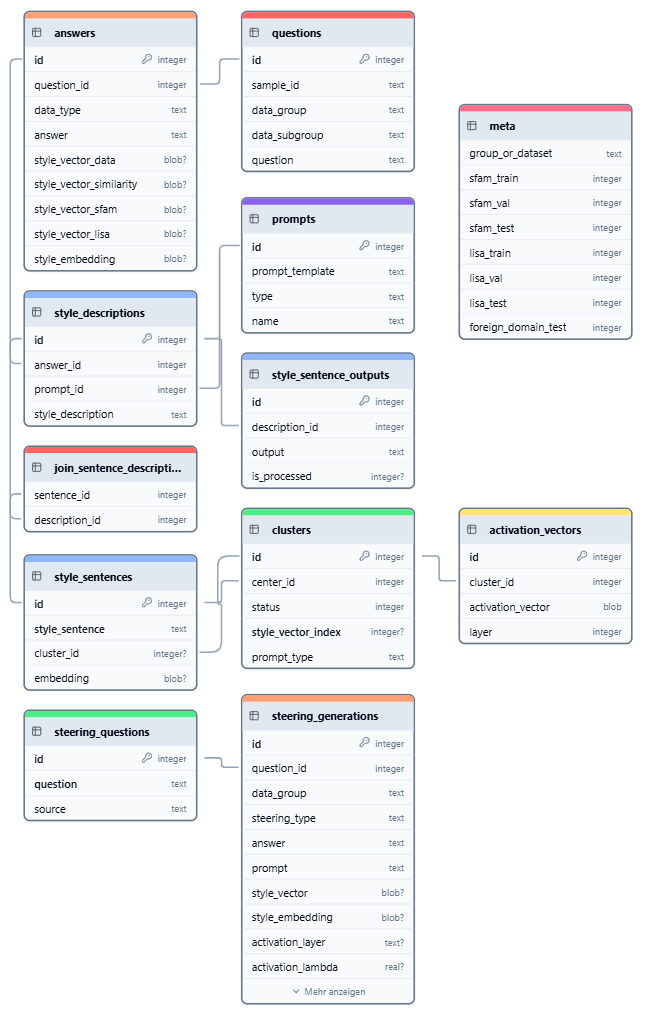
\includegraphics[width=\linewidth]{figures/sqlite-db.png}
\end{center}
       % INCLUDE: appendix
%
{%
    % if you are using zotero with the better bibtex plugin,
    % you can use the following postscript to automatically add the keyword 'preprint' for arXiv papers
    % (you find the postscript in the export tab of the Better BibTeX preferences, subtab postscript)
    % https://retorque.re/zotero-better-bibtex/exporting/scripting/
    % 
    % if (Translator.BetterBibLaTeX) {
    %     if (zotero.itemType === 'preprint') {
    %         const keyword = 'preprint';
    %         // Retrieve existing keywords, if any
    %         let keywords = zotero.tags.map(tag => tag.tag);
    %         // Add the 'preprint' keyword if it's not already present
    %         if (!keywords.includes(keyword)) {
    %             keywords.push(keyword);
    %             tex.add({ name: 'keywords', value: keywords, enc: 'tags' });
    %         }
    %     }
    % }

    \defbibfilter{websites}{
        type=online
        and not keyword=preprint
    }
    \defbibfilter{notWebsites}{
        not type=online
        or keyword=preprint
    }
    \setstretch{1.1}
    \renewcommand{\bibfont}{\normalfont\small}
    \setlength{\biblabelsep}{0pt}
    \setlength{\bibitemsep}{0.5\baselineskip plus 0.5\baselineskip}
    \printbibliography[filter=notWebsites]
    \newrefcontext[labelprefix={@}]
    \printbibliography[heading=subbibliography,title={Webpages},filter=websites]
}
\clearpage

%
% !TEX root = ../my-thesis.tex
%
\pagestyle{empty}
\hfill
\vfill
\pdfbookmark[0]{Colophon}{Colophon}
\section*{Colophon}

This thesis was typeset with \LaTeXe.
It uses the \textit{Clean Thesis} style developed by Ricardo Langner.

Download the \textit{Clean Thesis} style at \url{http://cleanthesis.der-ric.de/}.

% \clearpage


% \newpage
% \mbox{}

% **************************************************
% End of Document CONTENT
% **************************************************
\end{document}
